\documentclass[a4paper,12pt]{extarticle}
\renewcommand{\baselinestretch}{1.75} 

\usepackage[utf8]{inputenc}
\usepackage[left=0.9in,top=0.9in,right=0.9in,bottom=0.9in]{geometry}
\usepackage{amsmath}
\usepackage{amssymb}
\usepackage{amsthm}
\usepackage{graphicx}
\usepackage{mathptmx}
\usepackage{tabularx}
\usepackage{url}
\usepackage{caption}
\usepackage{subcaption}
\usepackage[
backend=biber,
style=numeric,
]{biblatex}
\addbibresource{reference.bib} %Imports bibliography file
\usepackage[TS1,T1]{fontenc}
% \usepackage{fourier, heuristica}
\usepackage{array, booktabs}
\usepackage{graphicx}
\usepackage[x11names,table]{xcolor}
\usepackage{titlesec}

\setlength{\parindent}{4em}
\setlength{\parskip}{1em}
\renewcommand{\arraystretch}{0.8}

\DeclareMathOperator*{\relu}{ReLU}

\titlespacing\section{0pt}{0pt plus 0pt minus 0pt}{0pt plus 0pt minus 0pt}
\titlespacing\subsection{0pt}{0pt plus 0pt minus 0pt}{0pt plus 0pt minus 0pt}
\titlespacing\subsubsection{0pt}{0pt plus 0pt minus 0pt}{0pt plus 0pt minus 0pt}


\begin{document}

\pagenumbering{gobble}

\begin{titlepage}
	\begin{center}
		\vspace*{0px}
		\small{H574160: Control Telerobotic Arm Remotely Via Pose Detection Of Human Arm}\\

		\vspace*{240px}
		\small{Submited By}\\
		\small{Ng Wei Jie, Brandon} \\
		\small{Department Of Electrical \& Computer Engineering}

		\vspace*{240px}
		\small{In Partial Fulfillment Of The}\\
		\small{Requirements For The Degree Of}\\
		\small{Bachelor Of Engineering}\\
		\small{National University Of Singapore}\\

	\end{center}
\end{titlepage}
\newpage

\begin{center}
    \large{\textbf{Abstract}}    
\end{center}
\noindent
This project explored an alternative approach to control the robotic arm remotely via gestures from 3D pose estimation on RGB images. 3D pose estimations were performed on the upper body and the hand to control the position and orientation of the end effector respectively.

\noindent
The 3D pose estimation models were designed and trained from scratch. A Resnet encoder-decoder architecture was trained on 2D poses. The encoder serves as an image embedding. A 3D pose module fuses the features in the image embedding from the encoder before passing to a stack of graph convolution layers and nonlocal layers to estimate the 3D poses.  

\noindent
The 3D pose estimation models were trained on open-sourced synthetic hand dataset and real hand dataset. The synthetic dataset generalised well on real data. Upper body pose dataset was self-collected. The same model was trained and evaluated on the self-collected dataset. Hyperparameters were experimented, including different loss functions, to achieve better performance.

\noindent
The 3D pose estimator models were integrated with a simulated and physical robotic arm to demonstrate the teleoperation. The robotic arm could teleoperate to some extent. A pick-and-place was performed to demonstrate the teleoperation.
\newpage

\tableofcontents
\newpage

\listoffigures
\listoftables
\newpage

\pagenumbering{arabic}
\section{Introduction}

\noindent
Human body and hand pose estimation plays an important role in gesture control. This task is challenging because multiple poses can be mapped to the same pose on the image. Besides, when the joints are occluded, it is difficult to reasonably estimate the pose \cite{poseestimationreview}. Pose estimation to remotely control a robotic arm via gestures is useful in operating tasks that are dangerous and physically demanding. Although Virtual Reality and Haptic Devices are commonly used, they are expensive and inconvenient for personal use \cite{shadowrobot, teleexistence}.

\noindent
To make the remote control of the robotic arm more accessible, pose estimations on the upper body and hand are investigated as an alternative approach. Pose estimation is performed on RGB images to extract 3D poses on the upper body and hand. The upper body pose is used to control the position of the robotic arm's gripper, while the lower body pose is used to control the orientation of the gripper and the gripper size. The gripper is the robot's end effector.

\section{Contributions}

\noindent
In this project, a new approach to control the robotic arm via gestures from pose estimation on RGB images is explored and demonstrated on a simulated and physical robot. Pose estimation models for the hand are designed with reference to related works, trained from scratch, and fine-tuned to become suitable for real-time inference. The same pose estimation model for the upper body is also trained using a dataset that was self-collected.


\newpage
\section{Related Works}
\noindent
3D pose estimation is the problem of estimating the 3D joint locations from an image frame. Earlier methods attempt to predict the 3D poses from a volumetric space; however, the accuracy  of the poses is limited by the output resolution \cite{poseestimationreview}. Current methods treat the task of estimating the 3D poses as a regression problem that is simpler and requires less computation \cite{poseestimationreview}. The pose estimation models can be trained to learn the joint locations from the image directly or can be trained using a separate lightweight network to learn the 3D poses from 2D poses \cite{baseline, poseestimationreview}. 

\noindent
The common issue in estimating 3D poses is the ambiguity in the mapping from 2D poses to 3D poses \cite{poseestimationreview}. There are methods that use temporal information of poses and multi-view frames to address this ambiguity \cite{poseestimationreview}. Since the image provides rich information about the 3D pose, several methods attempt to encode the image features to provide an embedding for the model to learn the 3D poses \cite{blazepose, handgcn, olha}. The encoded features were supervised by the ground truths of the 2D poses.

\noindent
The encoder-decoder architecture is a common architecture used in pose estimation models to encode information in the image \cite{olha}. Pose estimation models use this architecture to return 2D heat maps of the same size as the input images \cite{olha}. The heat maps indicate where the keypoints of the 2D poses are in the image. The encoder extracts information from the image and represent as an embedding \cite{blazepose}. The decoder uses the embedding to localise the keypoint in the image. Skip connections are also used to combine the high and low level information to obtain more precise decoding \cite{olha, blazepose}. This section primarily examines the works contributed by Chernytska, Bazarevsky, and Zhao that use the encoder-decoder architecture and are relevant to this paper \cite{blazepose, handgcn, olha}.

\noindent
Chernytska used a ResNet-based encoder-decoder architecture for 3D hand pose estimation models in 2019 \cite{olha}. The model used ResNet34 as the encoder. In ResNet34, the image passed through 1 convolution layer, followed by 4 residual layers where each layer is made of 3, 4, 6, 3 residual blocks respectively \cite{resnet}. In the decoder, 4 upsampling blocks were used where the input from the previous decoding layer is upsampled and concatenated with the input from the intermediate residual layers of the encoder \cite{olha}. The output from the last upsampling block is upsampled once more to return 2D heat-maps of the same size as the original image \cite{olha}. The peak of 2D heat-maps indicates where the keypoints of the 2D poses are in the image. To predict the keypoints for the 3D poses, the output from the first residual layer of the encoder is concatenated with the heatmaps and passed to a regression module \cite{olha}. The last layer of the regression module is a fully-connected layer of output size 3 \(\times\) the number of joints to estimate the x, y, and z coordinates for each joint \cite{olha}. The model was trained using 2 loss functions - one for the 2D heatmaps and one for the 3D keypoints \cite{olha}.

\noindent
ResNet is commonly used as the feature extractor in many deep learning computer vision tasks. ResNet contains residual blocks which has a stack of few convolution layers \cite{resnet}. Each block fits onto a residual mapping \cite{resnet}. The residual block also has a skip connection where element-wise addition is performed on the input of the block and the output of the last layer of the block \cite{resnet}.  Equation \ref{eq:residual_connection} shows the residual mapping where \(x\) denotes the input, \(F(x)\) denotes the residual mapping, and \(H(x)\) denotes the desired mapping \cite{resnet}. Kaiming mentioned that it is easier for a stack of a few layers to learn and push the error to zero in residual mapping instead of a network learning the desired network due to vanishing gradient \cite{resnet}.
\begin{equation}
F(x) = H(x) - x \label{eq:residual_connection}
\end{equation}
\noindent
Zhao proposed an improved graph convolution module - Semantic Graph Convolution (SemGCN) - for 3D body pose estimation in 2019 \cite{semgcn}. SemGCN represents the body pose as a graph where the nodes are the joints and edges are the bones \cite{semgcn}. The graph convolution operation is shown in Equation \ref{eq:modified_gcn_convolutional_operation_receptive_field} and is an adaption of Graph Convolution Network (GCN) \cite{semgcn}. In GCN, the input \(\mathbf{X}\) is transformed by a learnable matrix \(\mathbf{W}\) and multiplied by a normalized adjacency matrix \(\mathbf{A}\) to learn features from neighbouring nodes in the graph \cite{semgcn}. However, the same learnable matrix \(\mathbf{W}\) is applied across the graph and limits the internal representative of the graph \cite{semgcn}. Zhao introduced a second learnable matrix \(\mathbf{M}\) to encode information for the each sub-graph in GCN \cite{semgcn}. This forms the improved GCN - SemGCN \cite{semgcn}. In Zhao's paper, he proposed two types of SemGCN models. The first model used 4 blocks, each block has 2 SemGCN layers, to take in 2D keypoints and outputs 3D keypoints \cite{semgcn}. The second model used a pre-trained 2D model with  ResNet50 as the encoder \cite{semgcn}. The features from the intermediate residual layers and heatmaps are flatten, concatenated and passed to the SemGCN model to estimate the 3D keypoints \cite{semgcn}. Both SemGCN models are supervised by two loss functions - one for the 3D bone vector and one for the 3D keypoints \cite{semgcn}.
\begin{equation}
\mathbf{X}^{l+1}=\sigma(\mathbf{W}\mathbf{X}^{l}\rho_i(\mathbf{M}\odot\mathbf{A})) \label{eq:modified_gcn_convolutional_operation_receptive_field}
\end{equation}
\noindent
In SemGCN, Zhao also used non-local layers to learn non-local relationship between nodes in the graph \cite{semgcn}. The idea of non-local layers was first introduced by Wang for video classification to increase the receptive field of convolution layers without increasing the computation cost due to a larger kernel size \cite{nonlocal}. The non-local operation is described in Equation \ref{eq:non_local_operation} and \ref{eq:non_local_f_operation} \cite{nonlocal}. The function \(f\) computes the affinity or relative importance between two entities, influencing the information contribution by the entities at difference location in the image or graph \cite{nonlocal}. 
\begin{equation}
\overrightarrow{x_i}^{l+1}=\overrightarrow{x_i}^{l}+\frac{W_x}{K}\sum_{j=1}^{K}f(\overrightarrow{x_i}^{l},\overrightarrow{x_j}^{l}).g(\overrightarrow{x_J}^{l}) \label{eq:non_local_operation}
\end{equation}
\begin{equation}
f(\overrightarrow{x_i}^{l},\overrightarrow{x_j}^{l})=\relu(\mathbf{w}_f [\theta(\overrightarrow{x_i}^{l})||\phi(\overrightarrow{x_j}^{l})]) \label{eq:non_local_f_operation}
\end{equation}
\noindent
Bazarevsky proposed BlazePose as a lightweight 2D body pose estimation model for real-time inference on mobile devices in 2020 \cite{blazepose}. BlazePose is available in the MediaPipe Python package to use out of the box \cite{blazepose}. The model used an encoder-decoder architecture with skip connections at each stage of the network \cite{blazepose}. The exact model architecture is not specified in the paper. The decoder networks consists of 4 upsampling blocks and outputs heat maps and offset maps of size \(\frac{1}{4}\) the size of the original image \cite{blazepose}. The heat maps estimates where the 2D keypoints are located in the image while the offset maps estimates the offset of the joint position at the pixel to overcome the limitation of the heat maps output resolution. The encoder-decoder network is trained and supervised by the heat map loss function and offset map loss function \cite{blazepose}. The decoder is then removed, and the encoder is freezed and stacked with a regression network \cite{blazepose}. The encoder serves as a lightweight embeddings \cite{blazepose}. The encoder and regressor is trained to estimate the 2D keypoints and the visibility \cite{blazepose}. Bazarevsky mentioned that this approach is more scalable and computationally less intensive \cite{blazepose}. The output layer is a fully-connected layer and can be modified to include more attributes for each keypoints \cite{blazepose}. The model is trained on an in-house dataset that is restricted to poses where certain keypoints can confidently annotated, such as the hips and shoulders \cite{blazepose}.


\newpage
\section{Datasets}
\subsection{NTU Hand Dataset}
\noindent
The NTU hand dataset is primarily used to evaluate the hand pose estimation model \cite{handgcn}. This dataset is synthetically generated and provides annotations for 3D pose and 3D meshes \cite{handgcn}. Photorealistic textures and shape blending are applied on the hand model \cite{handgcn}. The dataset contains 500 common hand gestures captures from 1000 angles under 30 lightlights \cite{handgcn}. The dataset also contains hand of 5 skin colors and the images are composed with random backgrounds \cite{handgcn}. There are 315000 images for training and 60000 for testing \cite{handgcn}. 

\noindent
Figure \ref{fig:ntu_sample_data} shows a sample data from the NTU hand dataset. Although the image is synthetically generated, the hand is very realistic. This project removed the images where the palm faces away from the camera or the finger joints are mostly occluded. This is to reduce the network size to limit support for hand poses where the anchor points, such as the finger joints, are visible to some extent. 

\begin{figure}[ht]
    \begin{center}
        \begin{subfigure}[b]{0.35\textwidth}
            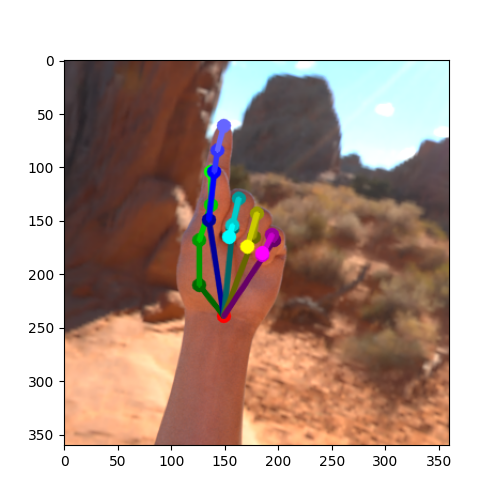
\includegraphics[width=150px]{assets/ntu_pose_2d.png}
            \caption{Pose 2D}
            \label{fig:ntu_pose_2d}
        \end{subfigure}
        \begin{subfigure}[b]{0.35\textwidth}
            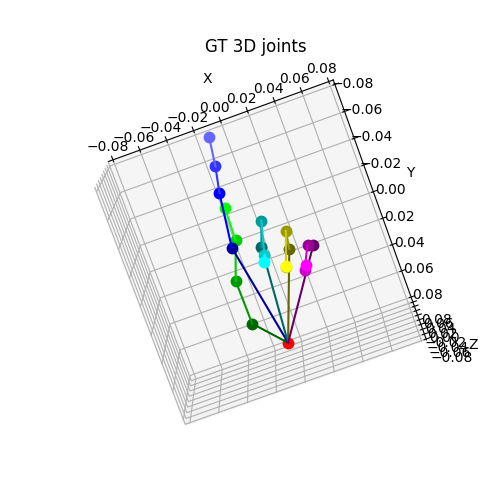
\includegraphics[width=150px]{assets/ntu_pose_3d.png}
            \caption{Pose 3D}
            \label{fig:ntu_pose_3d}
        \end{subfigure}
	    \caption{NTU Hand Data Sample}
	    \label{fig:ntu_sample_data}        
    \end{center}
\end{figure}

\newpage
\subsection{FreiHand Dataset}
\noindent
The Freihand is also used to evaluate the hand pose estimation model on real hands \cite{freihand}. A multi-view camera setup was setup to collect the hand poses and images without markers \cite{freihand}. The hand poses was collected from 32 subjects of different genders and ethic backgrounds, and they were tasked to perform actions with and without grasping objects \cite{freihand}. The hand poses were initially manually annotated, and a 3D model was trained on the existing dataset to predict and accelerate the fitting and annotation process \cite{freihand}.

\noindent
Figure \ref{fig:freihand_sample_data} shows a sample data from freihand dataset. The images were taken indoor and outdoor since the multi-view camera setup was portable \cite{freihand}. The images taken indoors were taken with a green background and augmented with random background by replacing the green pixels \cite{freihand}. This project removed the background augmented pictures because it does not generalises well to the outdoor images when the 2D pose estimation model was trained.
\begin{figure}[ht]
    \begin{center}
        \begin{subfigure}[b]{0.35\textwidth}
            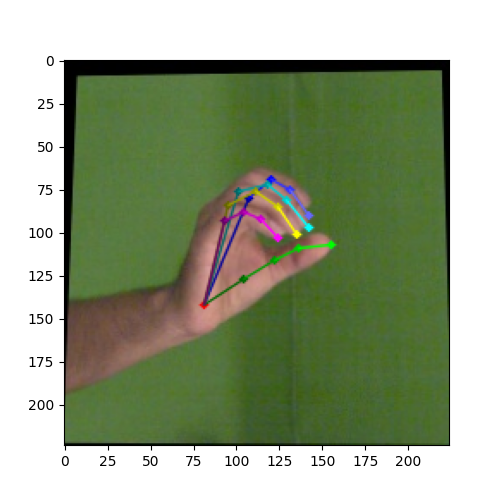
\includegraphics[width=150px]{assets/freihand_pose_2d.png}
            \caption{Pose 2D}
            \label{fig:freihand_pose_2d}
        \end{subfigure}
        \begin{subfigure}[b]{0.35\textwidth}
            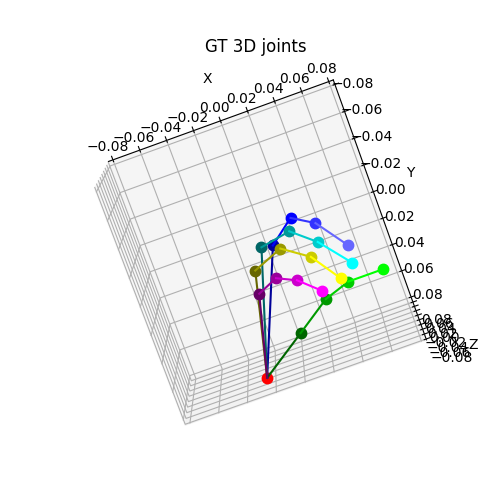
\includegraphics[width=150px]{assets/freihand_pose_3d.png}
            \caption{Pose 3D}
            \label{fig:freihand_pose_3d}
        \end{subfigure}
	    \caption{Freihand Data Sample}
	    \label{fig:freihand_sample_data}        
    \end{center}
\end{figure}


\newpage
\subsection{Custom Upper Body Dataset}
\noindent
An upper body pose estimation model is trained to provide the 3D position for the end effector of the robot. The pose estimation model is trained and evaluated on a custom dataset that was collected using a depth camera - Intel Realsense D455. The setup is shown in Figure \ref{fig:body_pose_data_collection_setup}. The distance from the joint to the camera is obtained from the depth image.

\begin{figure}[ht]
	\begin{center}
		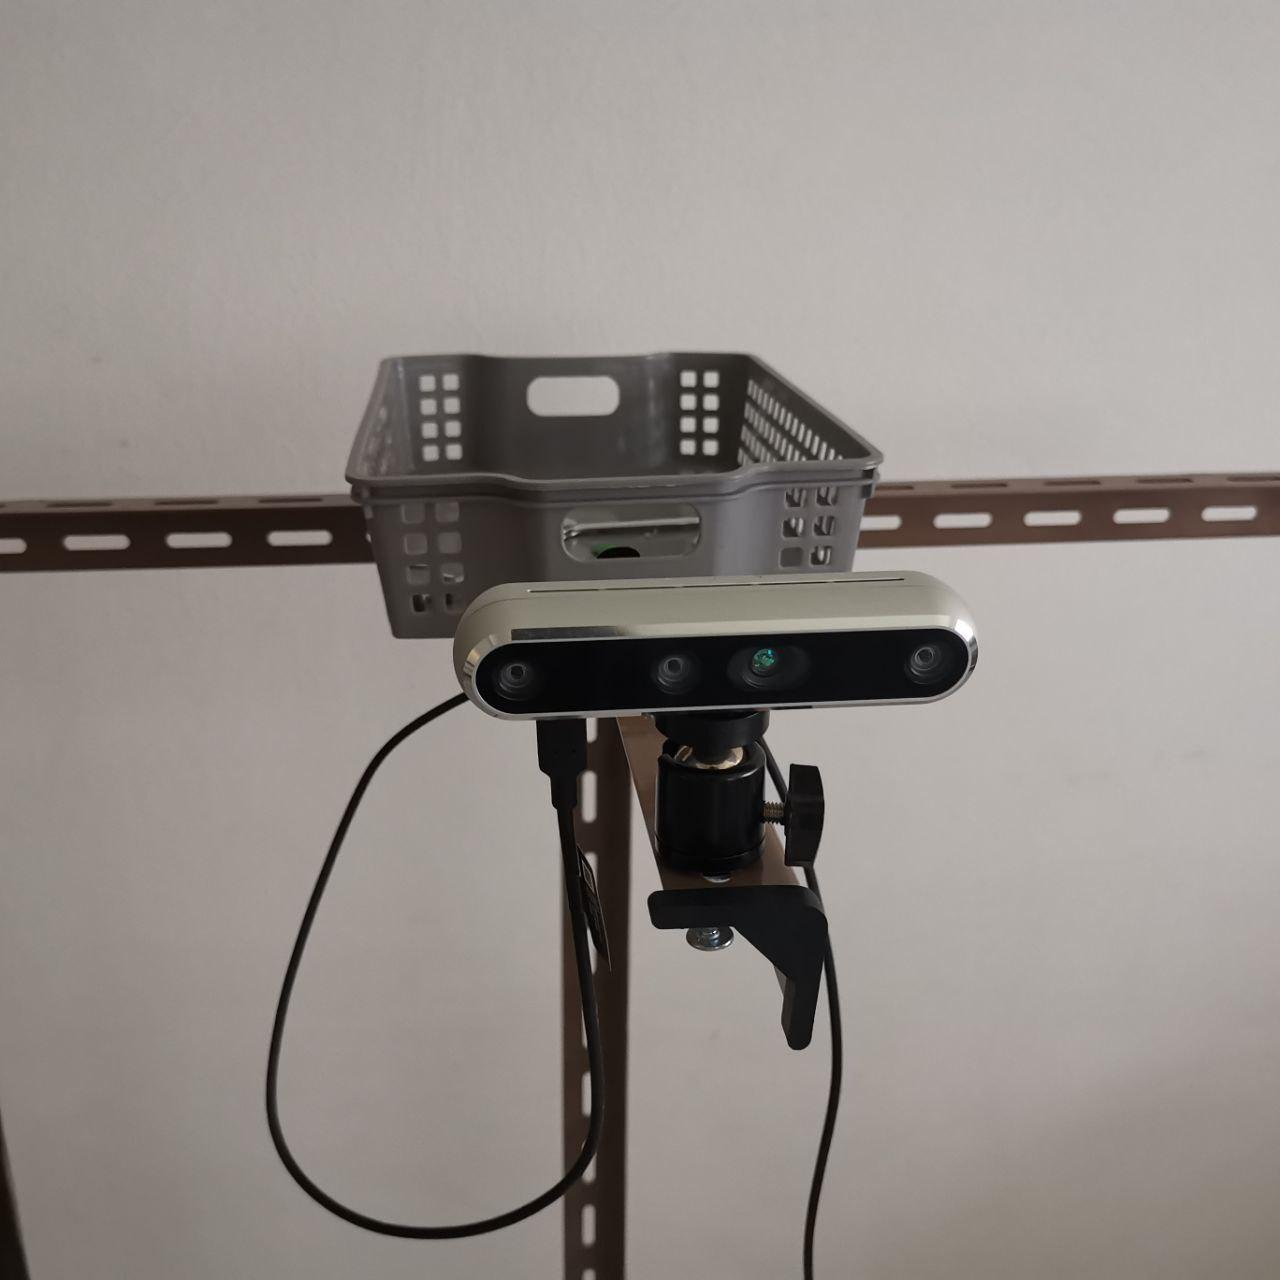
\includegraphics[width=100px]{assets/body_pose_setup.jpg}
		\caption{Body Pose Data Collection Setup}
		\label{fig:body_pose_data_collection_setup}
	\end{center}
\end{figure}

\noindent
Figure \ref{fig:custom_sample_data} shows a sample data of the upper body pose dataset. A lightweight pose 2D estimation model inferred the 2D keypoints to obtain the pixel coordinate \cite{lightweightopenpose}. The 3D pose was computed from the measured depth and camera intrinsic. If the depth image failed to measure the distance or the keypoints are occluded, the nearest pixel with a valid depth is searched. The data is collected for 10 different actions, and 3 different background for training and 2 different background for testing. There are 90000 images for training and 10000 for testing.

\begin{figure}[ht]
    \begin{center}
        \begin{subfigure}[b]{0.35\textwidth}
            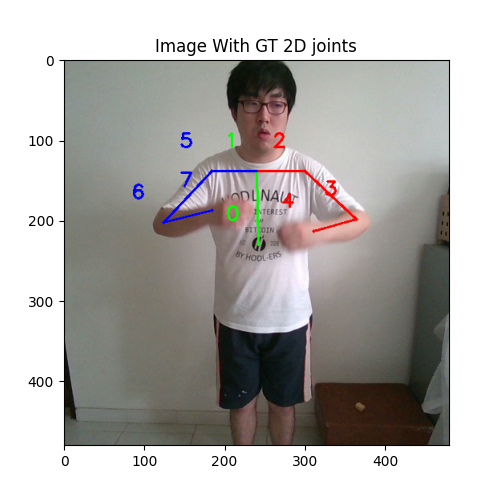
\includegraphics[width=150px]{assets/custom_pose_2d.png}
            \caption{Pose 2D}
            \label{fig:custom_pose_2d}
        \end{subfigure}
        \begin{subfigure}[b]{0.35\textwidth}
            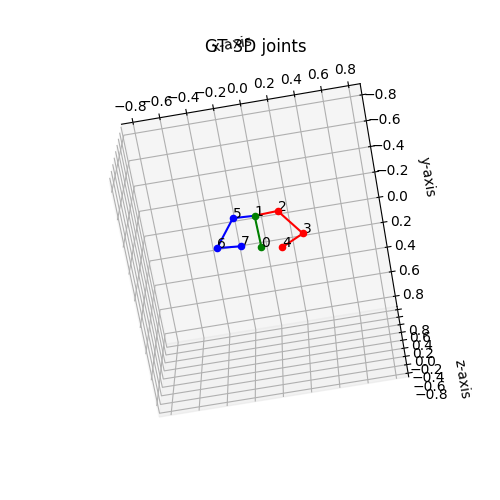
\includegraphics[width=150px]{assets/custom_pose_3d.png}
            \caption{Pose 3D}
            \label{fig:custom_pose_3d}
        \end{subfigure}
	    \caption{Custom Upper Body Data Sample}
	    \label{fig:custom_sample_data}        
    \end{center}
\end{figure}


\newpage
\section{Experimentation}
\subsection{Data Augmentation}
\noindent
Data augmentation is performed on images of the hand and upper body poses to reduce the model overfitting. This helps in generalising on a variety of poses better. Table \ref{table:augmentation_step} shows the augmentation steps performed on the poses and images. Flipping and mirroring is not performed for the upper body pose since the upper body is symmetric to some extent. All the joints of the hand and body pose are within the image after rotation and translation.

\begin{table}[ht]
\centering
\begin{tabular*}{\textwidth}{c @{\extracolsep{\fill}} p{2.5in} cc}
\hline
Augmentation Step & \centering Description & Hand Pose & Upper Body Pose \\ [0.5ex] 
\hline
Brightness & Adjusted image brightness by a factor in the range of [-0.25, 0.25] & Yes & Yes \\ 
Contrast & Adjusted image contrast by a factor in the range of [-0.25, 0.25] & Yes & Yes  \\
Sharpness & Adjusted image sharpness by a factor in the range of [-0.25, 0.25] & Yes & Yes \\
Mirror & Mirror original image & Yes & No \\
Flip & Flip original image & Yes & No \\
Rotate & Rotate by an angle in the range of [0, 360) degrees & Yes & Yes \\
Translate & Translate by a pixel in the range of [-100, 100] pixels & Yes & Yes  \\ 
Fill holes & Fill black pixels after transformation with background images & Yes & Yes  \\ 
[1ex] 
\hline
\end{tabular*}
\caption{Augmentation Steps}
\label{table:augmentation_step}
\end{table}
\noindent
The rotation step in the data augmentation is given in Equation \ref{eq:rotation_data_augmentation}. The rotation matrix is applied on the 3D keypoints to rotate the 3D pose and 2D pose about the z-axis.
\begin{equation}
\mathbf{P_{rotated}} = \begin{bmatrix}
cos(\theta) & -sin(\theta) & 0\\
sin(\theta) & cos(\theta) & 0\\
0 & 0 & 1
\end{bmatrix}
\mathbf{P}\label{eq:rotation_data_augmentation}
\end{equation}
\noindent
The translation step in the data augmentation is given in Equation \ref{eq:translation_x_data_augmentation} and \ref{eq:translation_y_data_augmentation}. \(p_{x}\) and \(p_{y}\) refers to the translation of 2D keypoints in the image and is measured in pixels. Similar triangles is applied to compute the translation of 3D keypoints.
\begin{equation}
x_{new} = x_{old} - \frac{p_x}{f_x} \times z \label{eq:translation_x_data_augmentation}
\end{equation}
\begin{equation}
y_{new} = y_{old} - \frac{p_y}{f_y} \times z \label{eq:translation_y_data_augmentation}
\end{equation}

\newpage
\subsection{Experimented Models}
\noindent
For this project, 4 different models were designed and experimented. The models were then modified to finetune the hyperparameters.

\noindent
The first model follows Chernytska and Zhaos' methods for encoder-decoder architecture of the 2D pose estimation model \cite{olha, semgcn}. A ResNet34 is used as the encoder. Skip connections are used in the decoder to concatenate the image embedding and the decoded information to obtain the heat maps. The 3D pose regressor follows Bazarevsky's high-level architecture \cite{blazepose}; however, the exact architecture is unknown. As a first attempt, each module in the regressor consists of a convolution layer and a residual block. This gives the model the complexity while avoiding the vanishing gradient problem. The heat maps and encoded information of the residual layers provide information to estimate the 3D poses. The last layer is a fully-connected layer and has an output size of 63 for x, y, and z coordinates for the 21 keypoints. The model architecture is shown in Figure \ref{fig:model_v1}.

\begin{figure}[ht]
	\begin{center}
		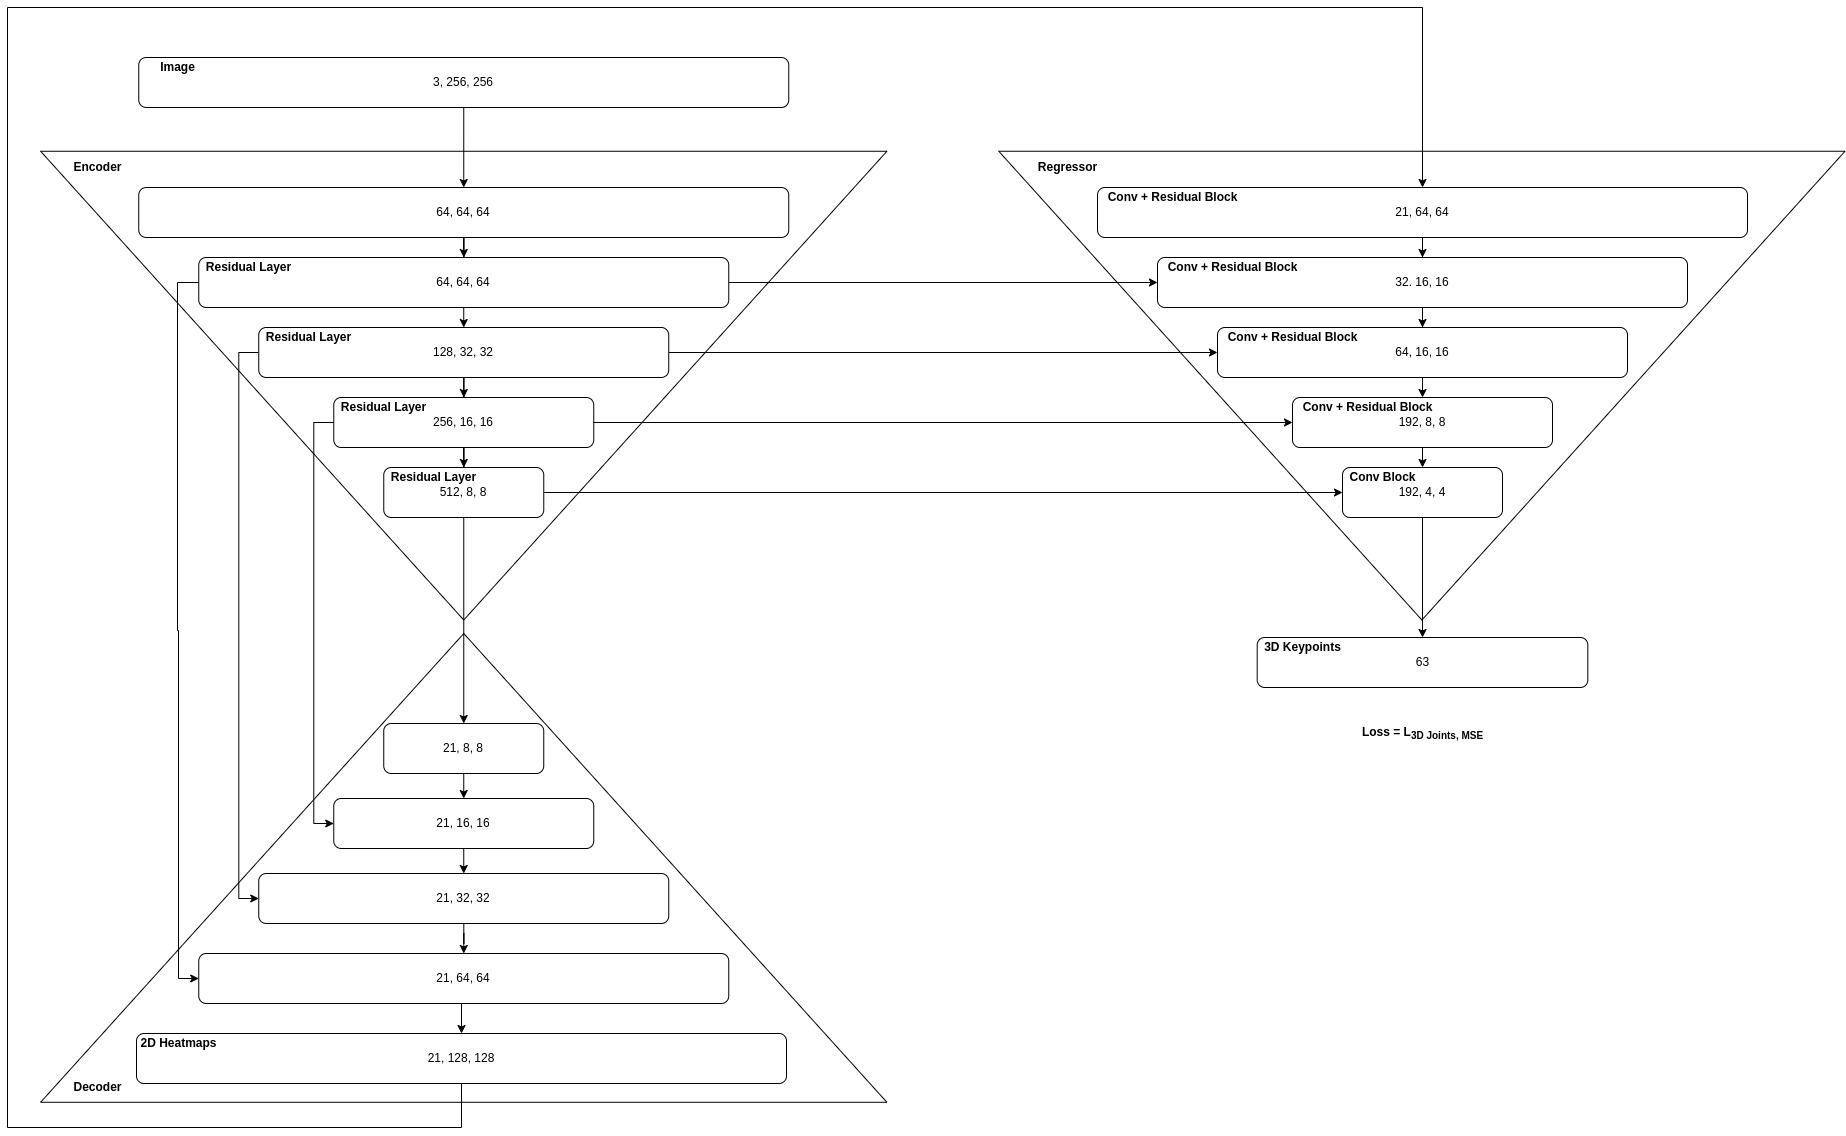
\includegraphics[width=450px]{assets/Model_v1.jpg}
		\caption{Model v1}
		\label{fig:model_v1}
	\end{center}
\end{figure}

\newpage

\noindent
Since this project is concerned with the estimation of 3D poses, the hyperparameters of the regressor model are modified, keeping the encoder-decoder module the same. Figure \ref{fig:model_v1_x} shows 3 different modifications to Model v1. The top left regressor is the original version. The top right regressor removes the heat map layer to determine if the heat map provides any useful information in estimating the 3D poses. The bottom left regressor increases the number of output channels in each layer to determine if more channels can learn better features for the estimation. The bottom right regressor decreases the output channels in each layer instead to determine if the model can still perform with fewer parameters.

\begin{figure}[ht]
	\begin{center}
		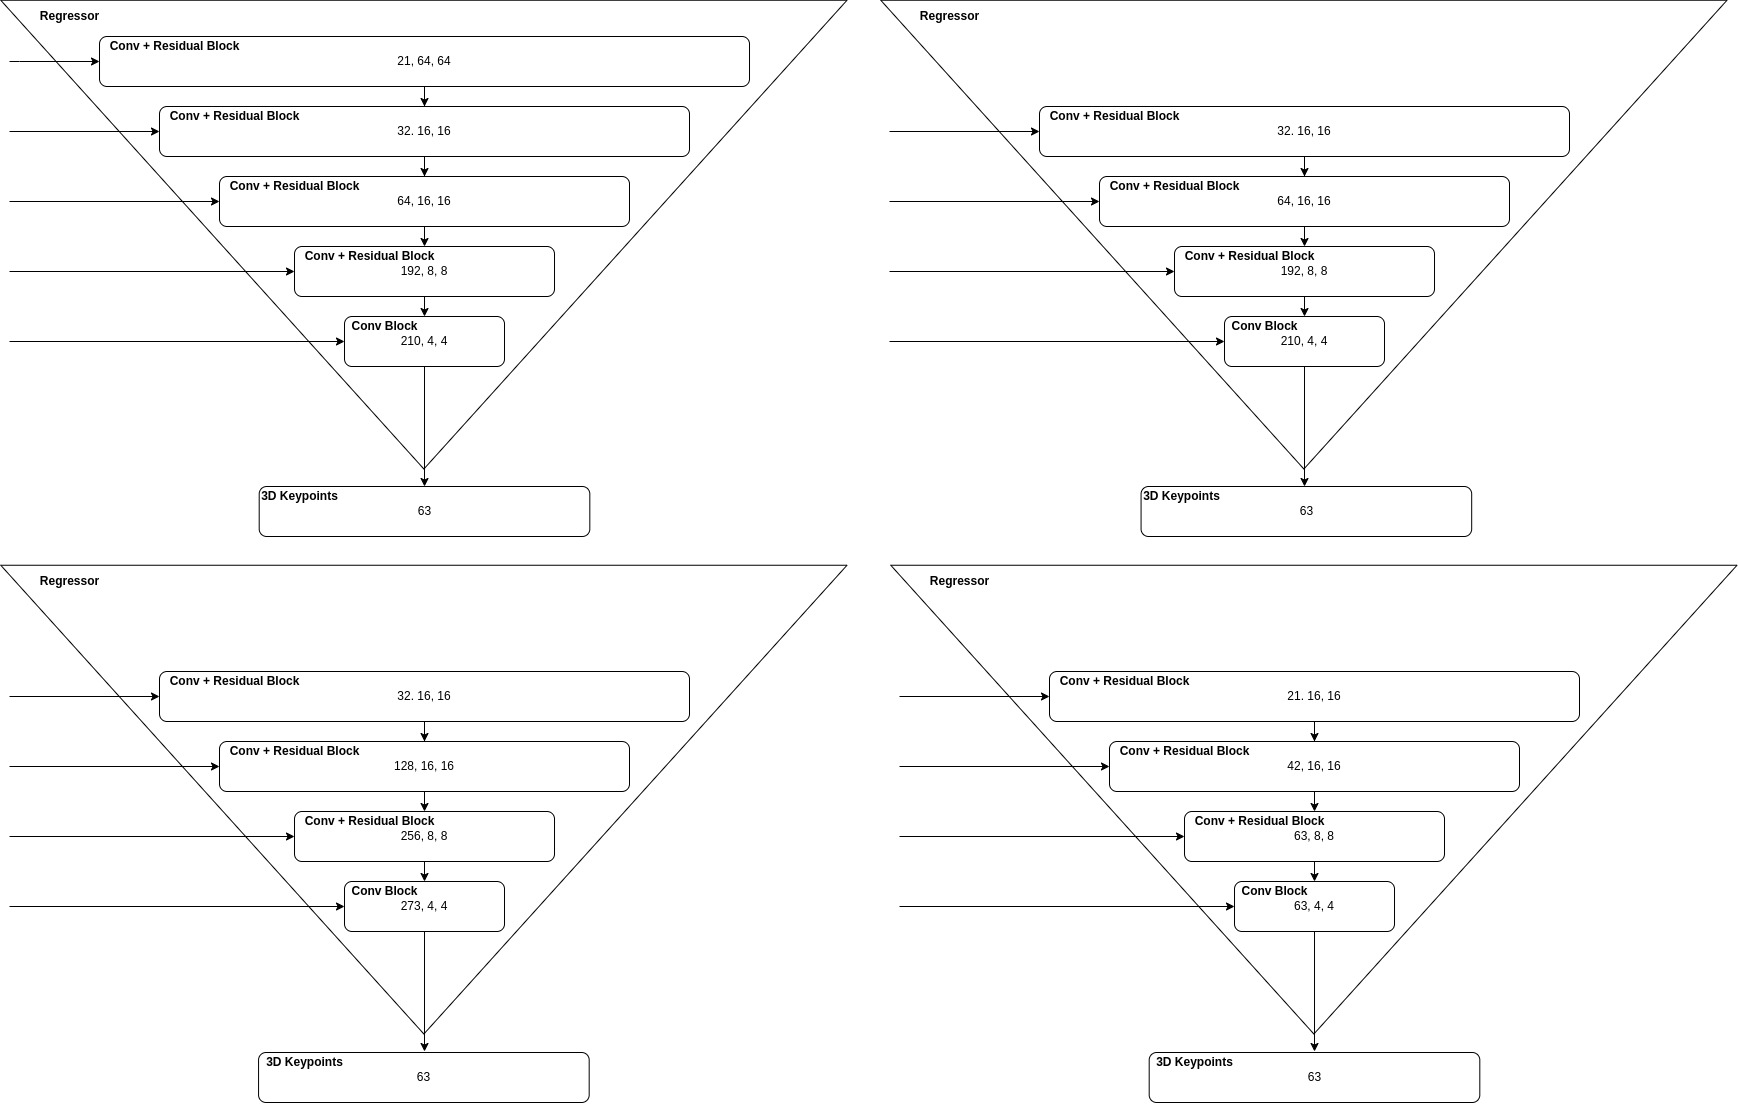
\includegraphics[width=450px]{assets/Model_v1.x.jpg}
		\caption{Hyperparameter Tuning For Model v1}
		\label{fig:model_v1_x}
	\end{center}
\end{figure}

\newpage

\noindent
The second model designed and experimented uses the same encoder-decoder architecture as the first model. The regressor model in the second model is almost the same as that of the first model except that each module in the regressor is using a convolution layer instead of a convolution layer and a residual block. This regressor model follows more closely with Bazarevsky's model if each stage in regressor model is a convolution layer (excluding the heat map). Similarly, the last layer is a fully-connected layer and has an output size of 63 for x, y, and z coordinates for the 21 keypoints. The model architecture is shown in Figure \ref{fig:model_v2}.

\begin{figure}[ht]
	\begin{center}
		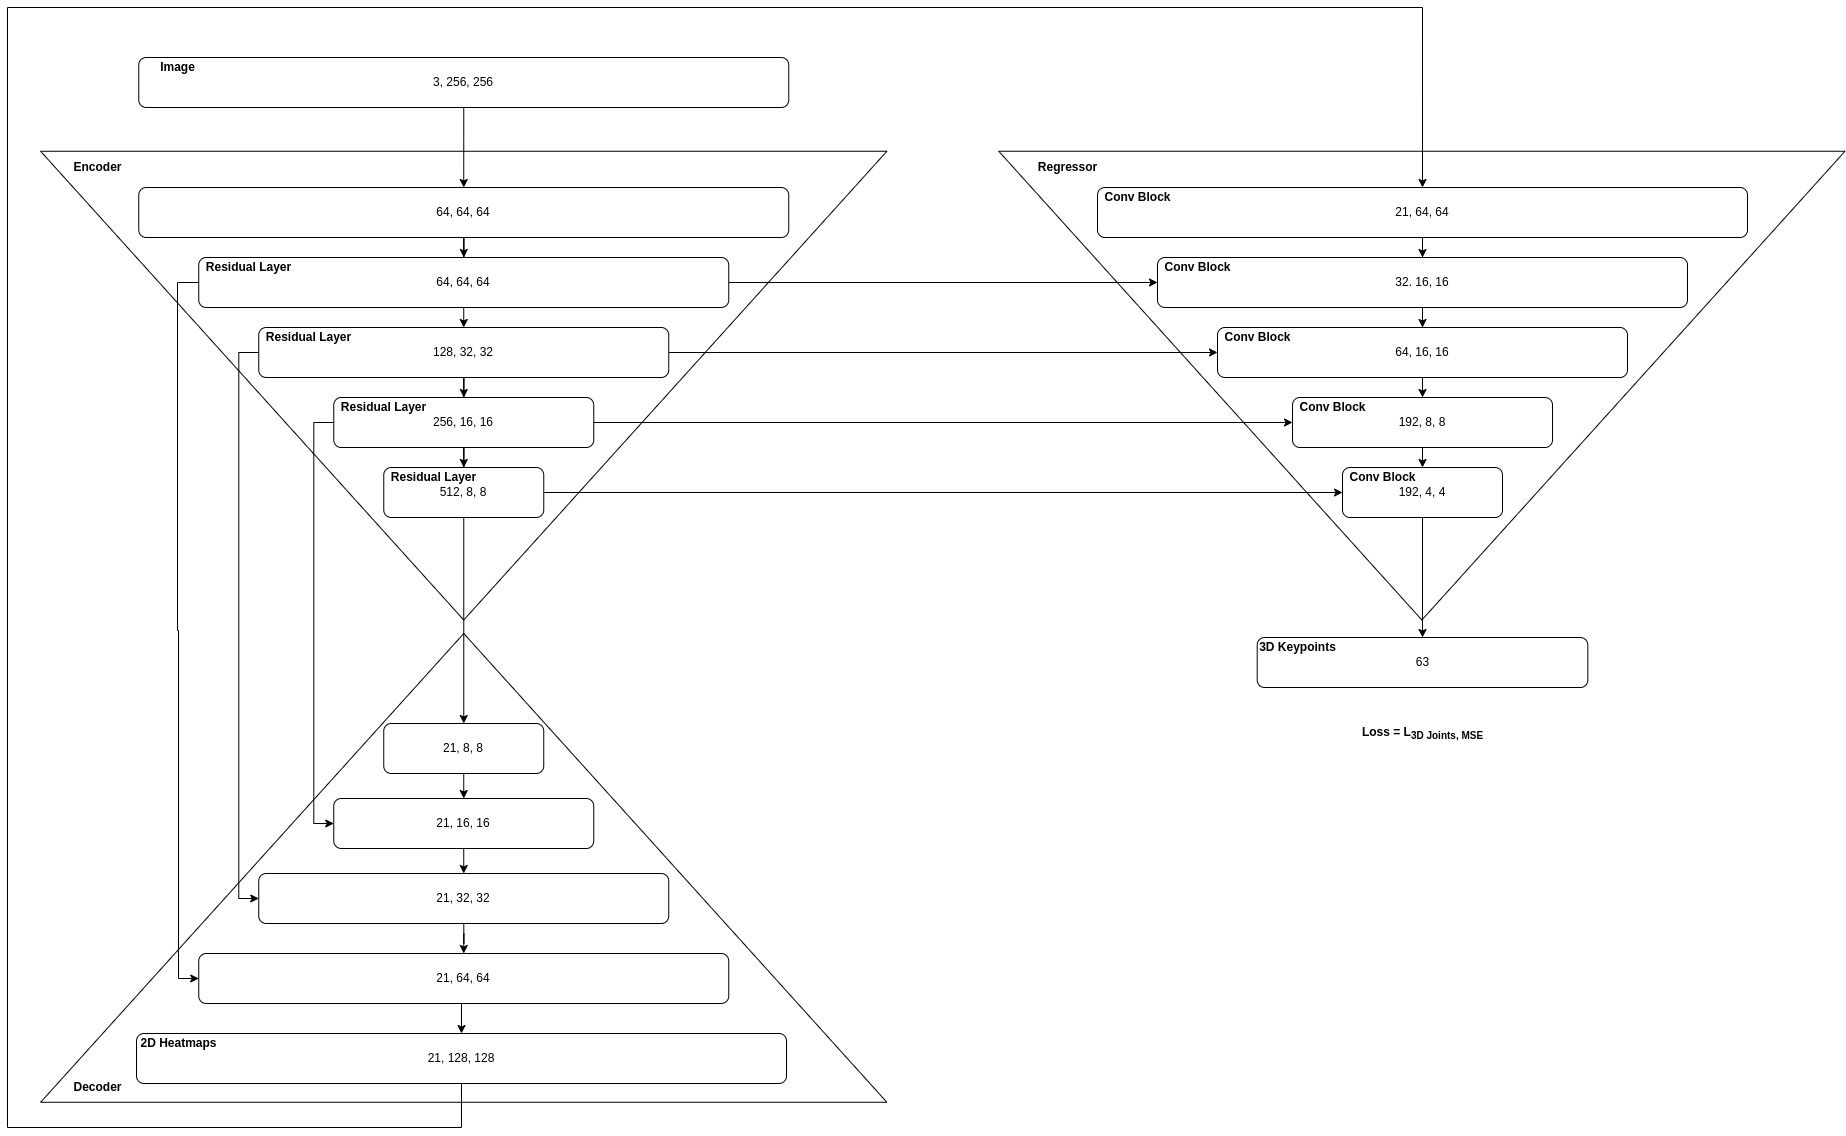
\includegraphics[width=450px]{assets/Model_v2.jpg}
		\caption{Model v2}
		\label{fig:model_v2}
	\end{center}
\end{figure}

\newpage

\noindent
The hyperparameters of the second model are modified, keeping the encoder-decoder modules the same. Figure \ref{fig:model_v2_x} shows 3 different modifications to Model v2. The top left regressor is the original version. The top right regressor removes the heat map layer to similarly determine if the heat map provides any useful information in estimating the 3D poses. The bottom left regressor increases the number of output channels in each layer to similarly determine if more channels can learn better features for the estimation. The bottom right regressor decreases the output channels in each layer instead to similarly determine if the model can still perform with fewer parameters. Like the first model, the same set hyperparameters were modified in the second model to concur the impact on the performance.

\begin{figure}[ht]
	\begin{center}
		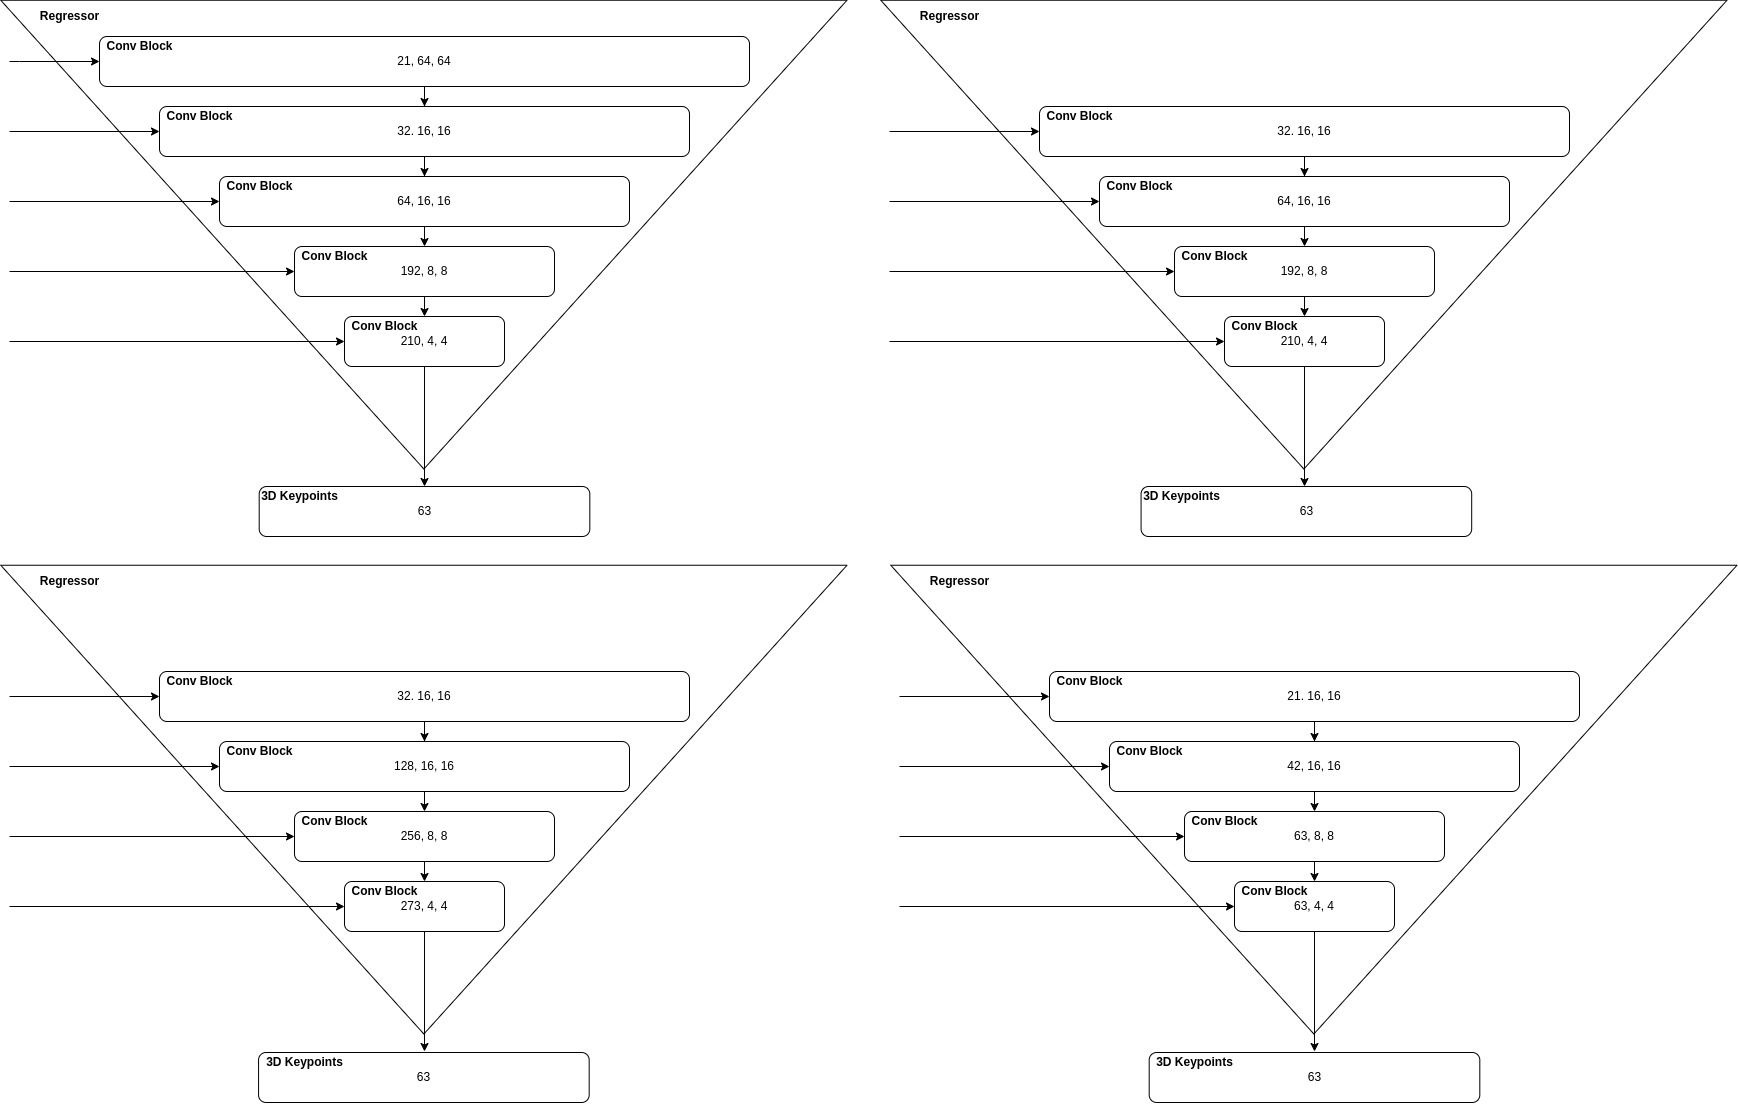
\includegraphics[width=450px]{assets/Model_v2.x.jpg}
		\caption{Hyperparameter Tuning For Model v2}
		\label{fig:model_v2_x}
	\end{center}
\end{figure}

\newpage

\noindent
The third model designed and experimented uses the same encoder-decoder architecture as the first and second model. The third model also used the same regressor model as the second model where each module is a convolution block. Only the final fully-connected layer is replaced with Zhao's SemGCN to estimate the 3D poses \cite{semgcn}. Zhao's proposed a similar architecture, but flatten the image embedding of the residual layers and heat maps as inputs to SemGCN \cite{semgcn}. In this SemGCN, non-local layers are also used to learn the distant relationship between two entities in the graph \cite{semgcn, nonlocal}. The SemGCN layers are repeated 4 times. This model will determine if graph convolution layers give better performance than using a fully-connected layer. The model architecture is shown in Figure \ref{fig:model_v3}. Note that the output channel in the last module of the regressor is different and is a multiple of the number of keypoints to resize to a valid tensor.

\begin{figure}[ht]
	\begin{center}
		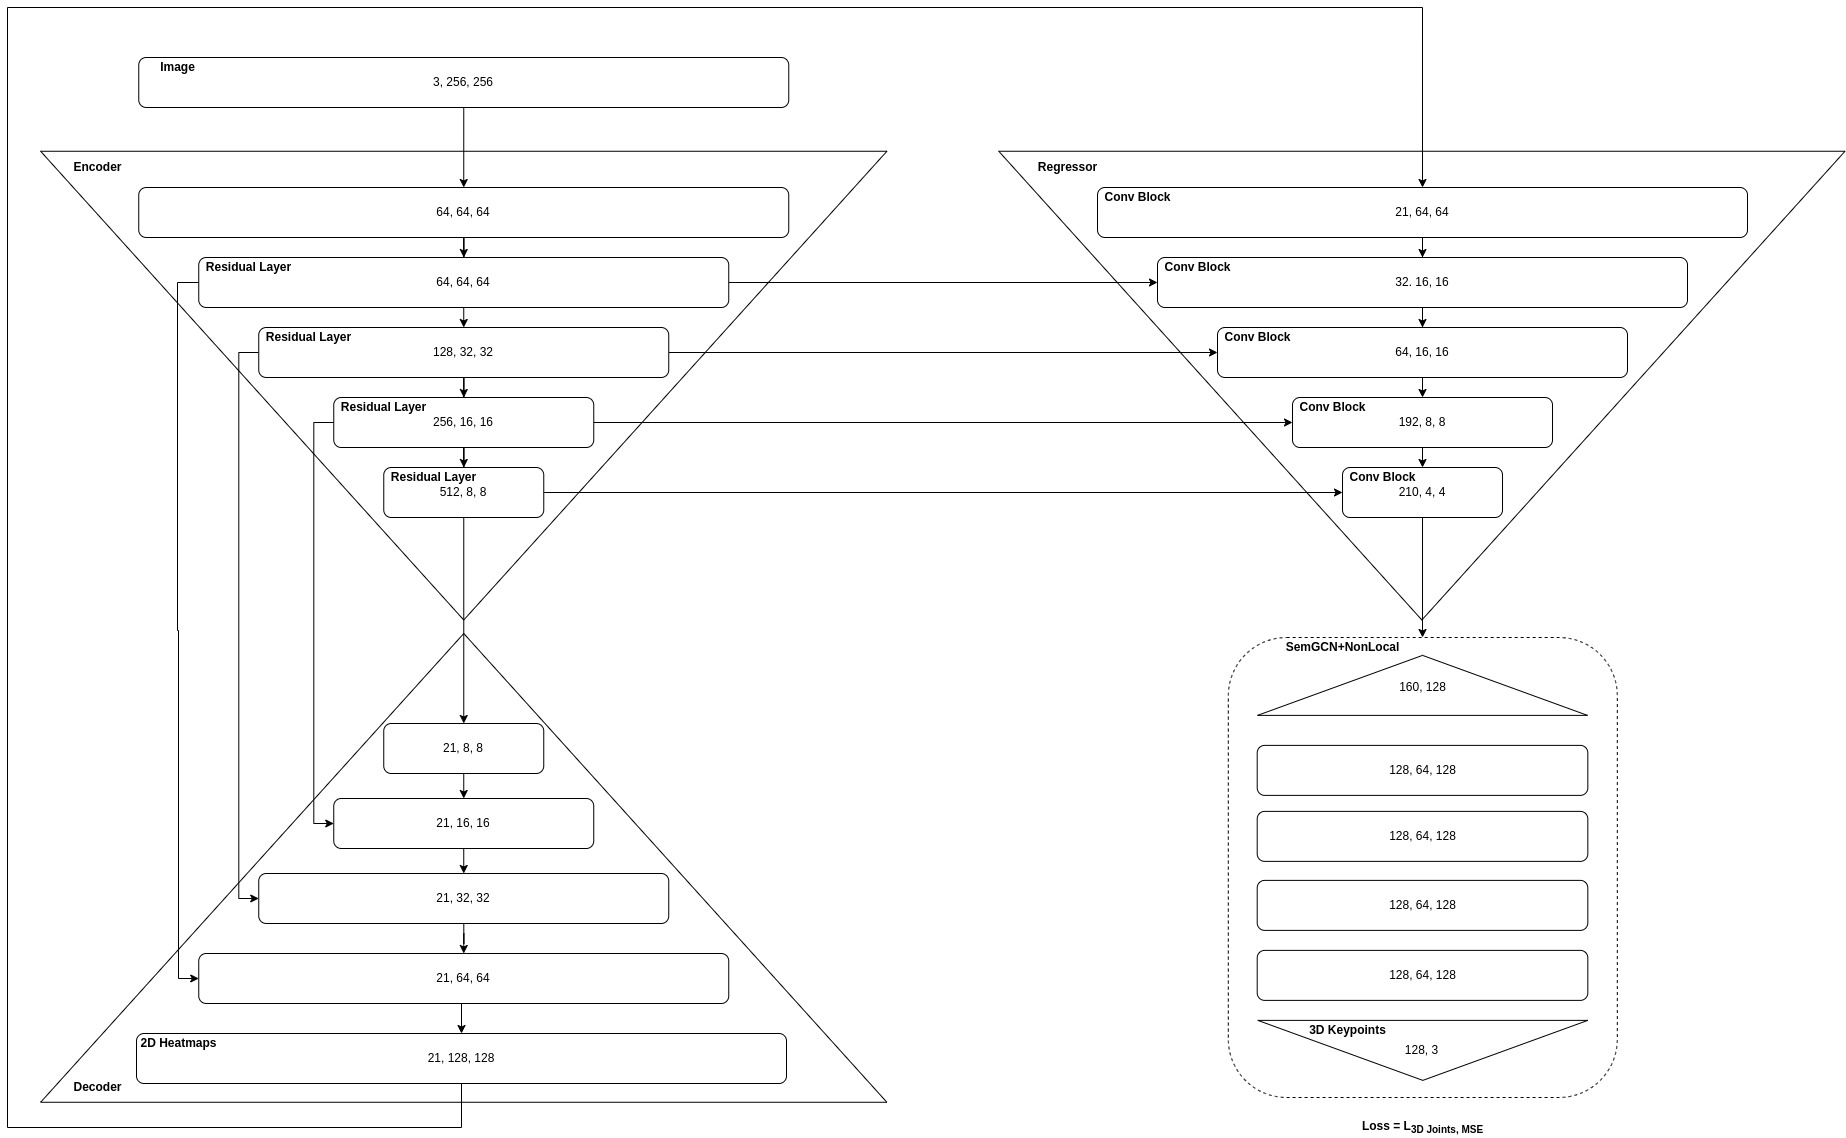
\includegraphics[width=450px]{assets/Model_v3.jpg}
		\caption{Model v3}
		\label{fig:model_v3}
	\end{center}
\end{figure}

\newpage

\noindent
The hyperparameters of the third model are modified, keeping the encoder-decoder module the same. Figure \ref{fig:model_v3_x} shows 3 different modifications to Model v3. The top left regressor is the original version. The top right regressor removes the heat map layer, the bottom left regressor increases the number of output channels in each layer, and the bottom right regressor decreases the output channels in each layer. Like the first and second model, the same set hyperparameters were modified in the third model to concur the impact on the performance.

\begin{figure}[ht]
	\begin{center}
		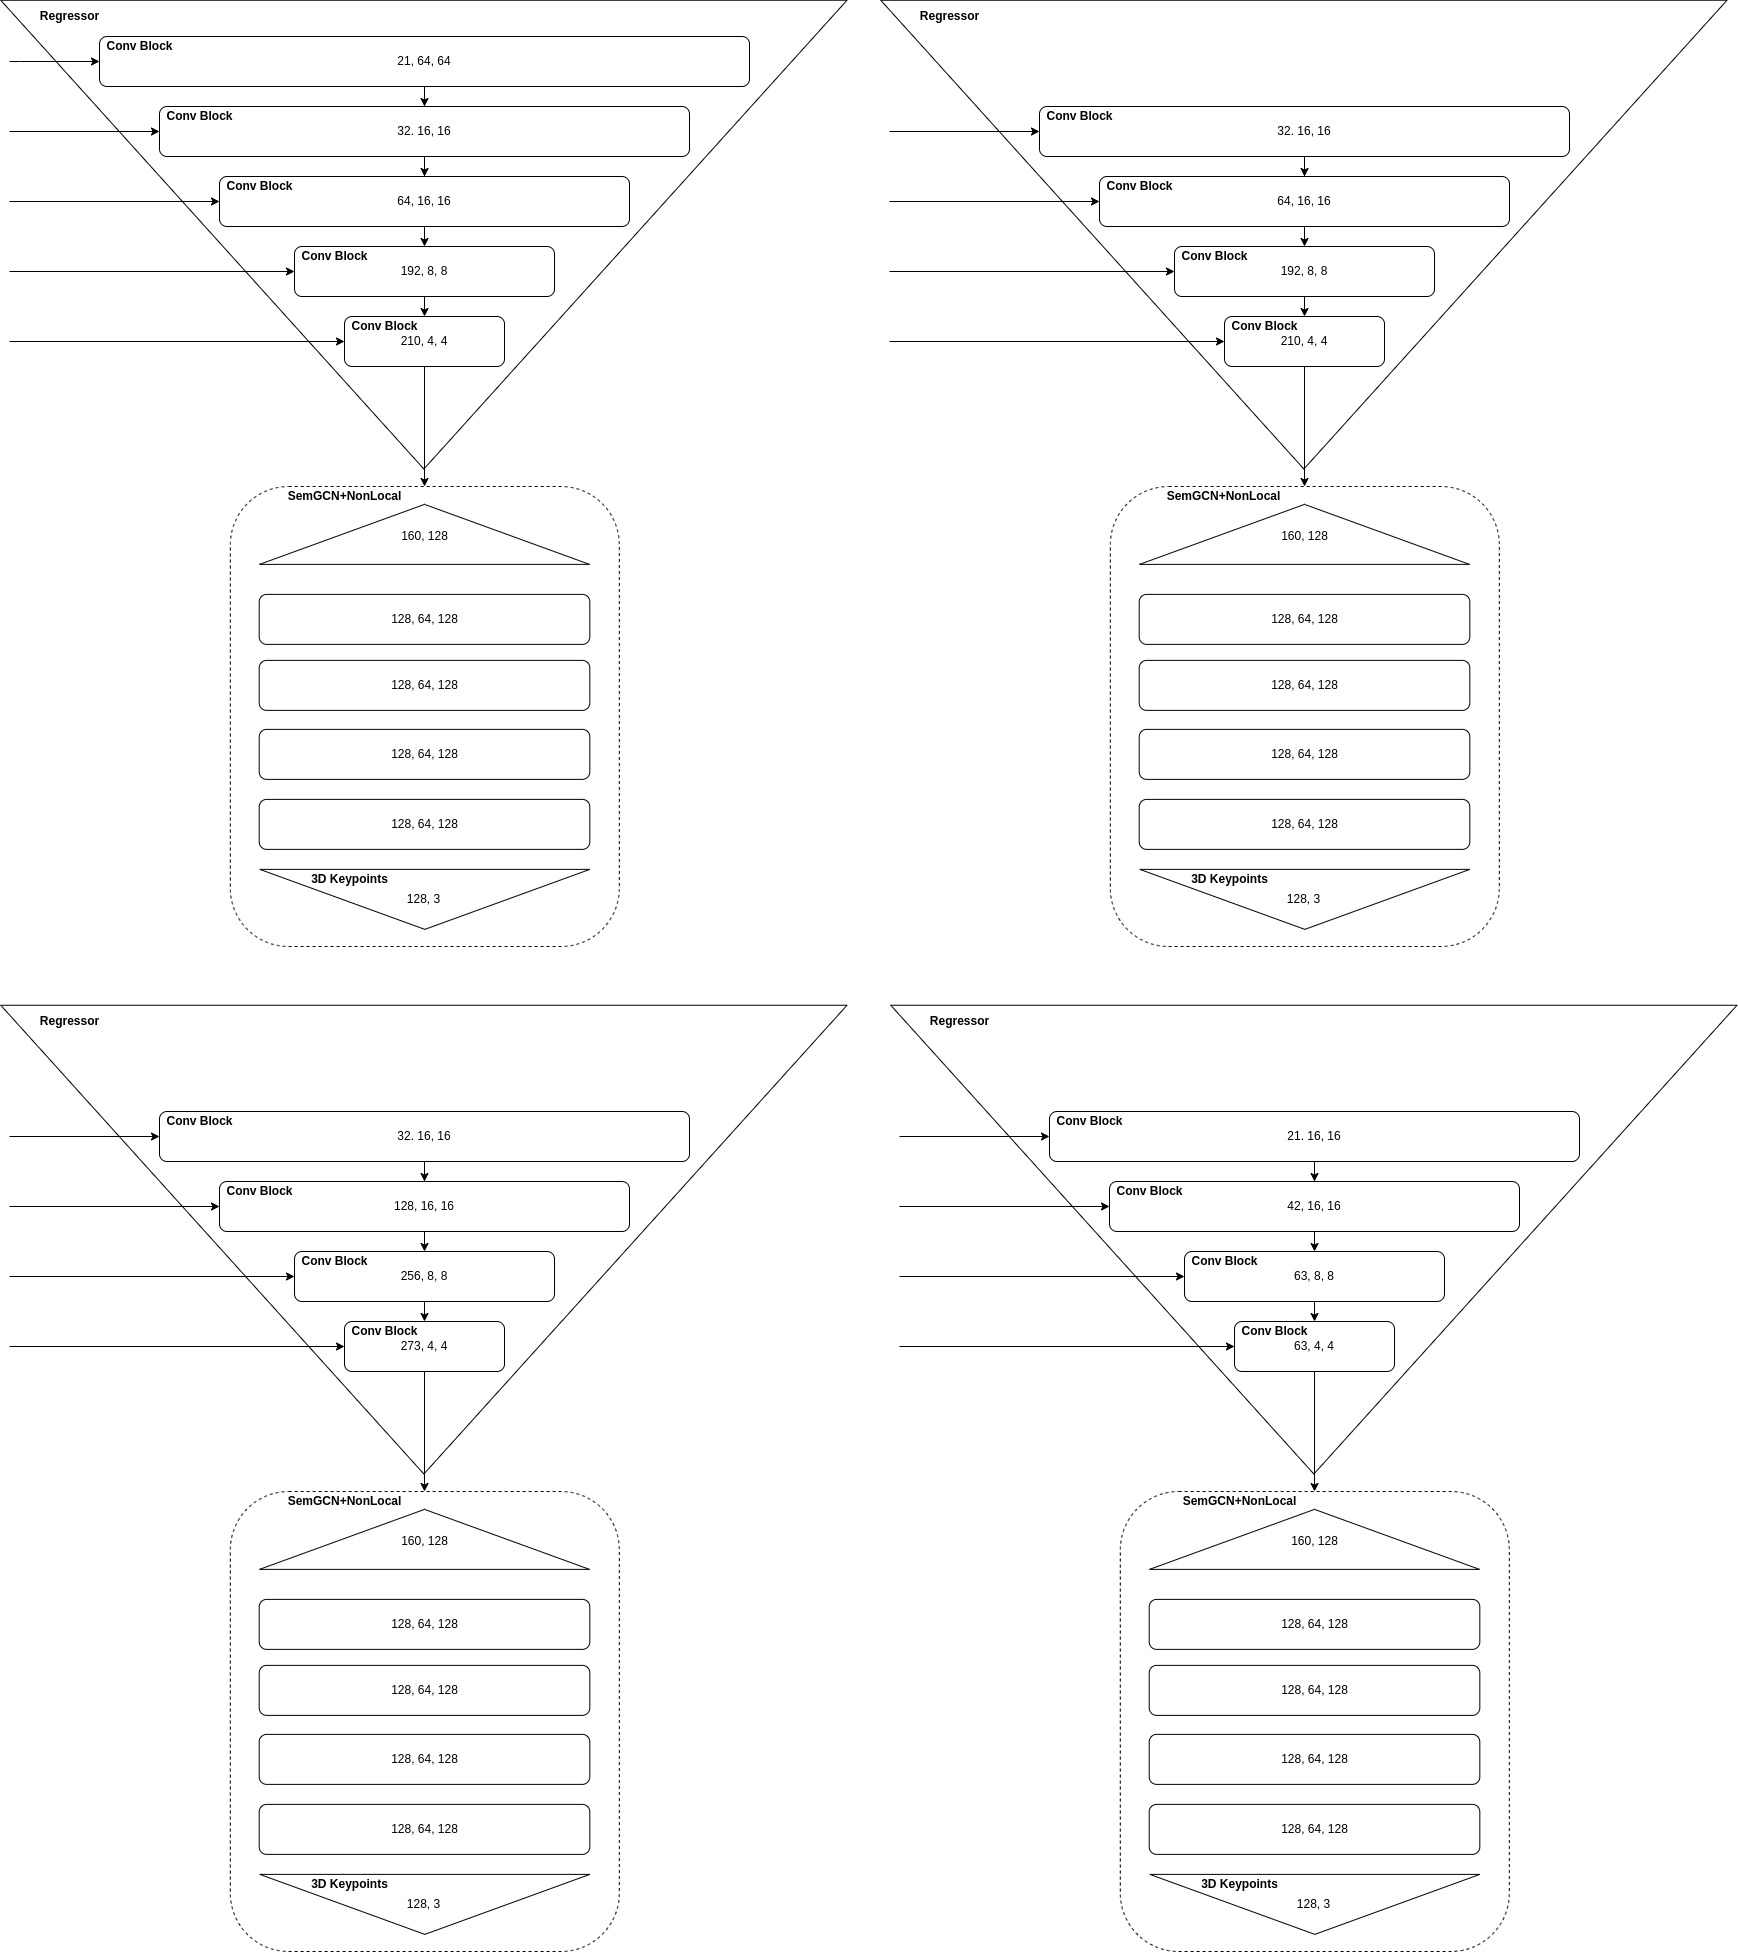
\includegraphics[width=450px]{assets/Model_v3.x.jpg}
		\caption{Hyperparameter Tuning For Model v3}
		\label{fig:model_v3_x}
	\end{center}
\end{figure}

\newpage

\noindent
The fourth model designed and experimented uses the same encoder-decoder architecture as the first, second, and third model. The fourth model also used the same regressor model as the third model where each module is a convolution block and SemGCN layers are used instead of a fully-connected layer. However, non-local layers are not used in this model to determine if the non-local layers can help the model estimate the 3D poses better if distant relationship between two entities in the graph are learnt. The model architecture is shown in Figure \ref{fig:model_v4}.

\begin{figure}[ht]
	\begin{center}
		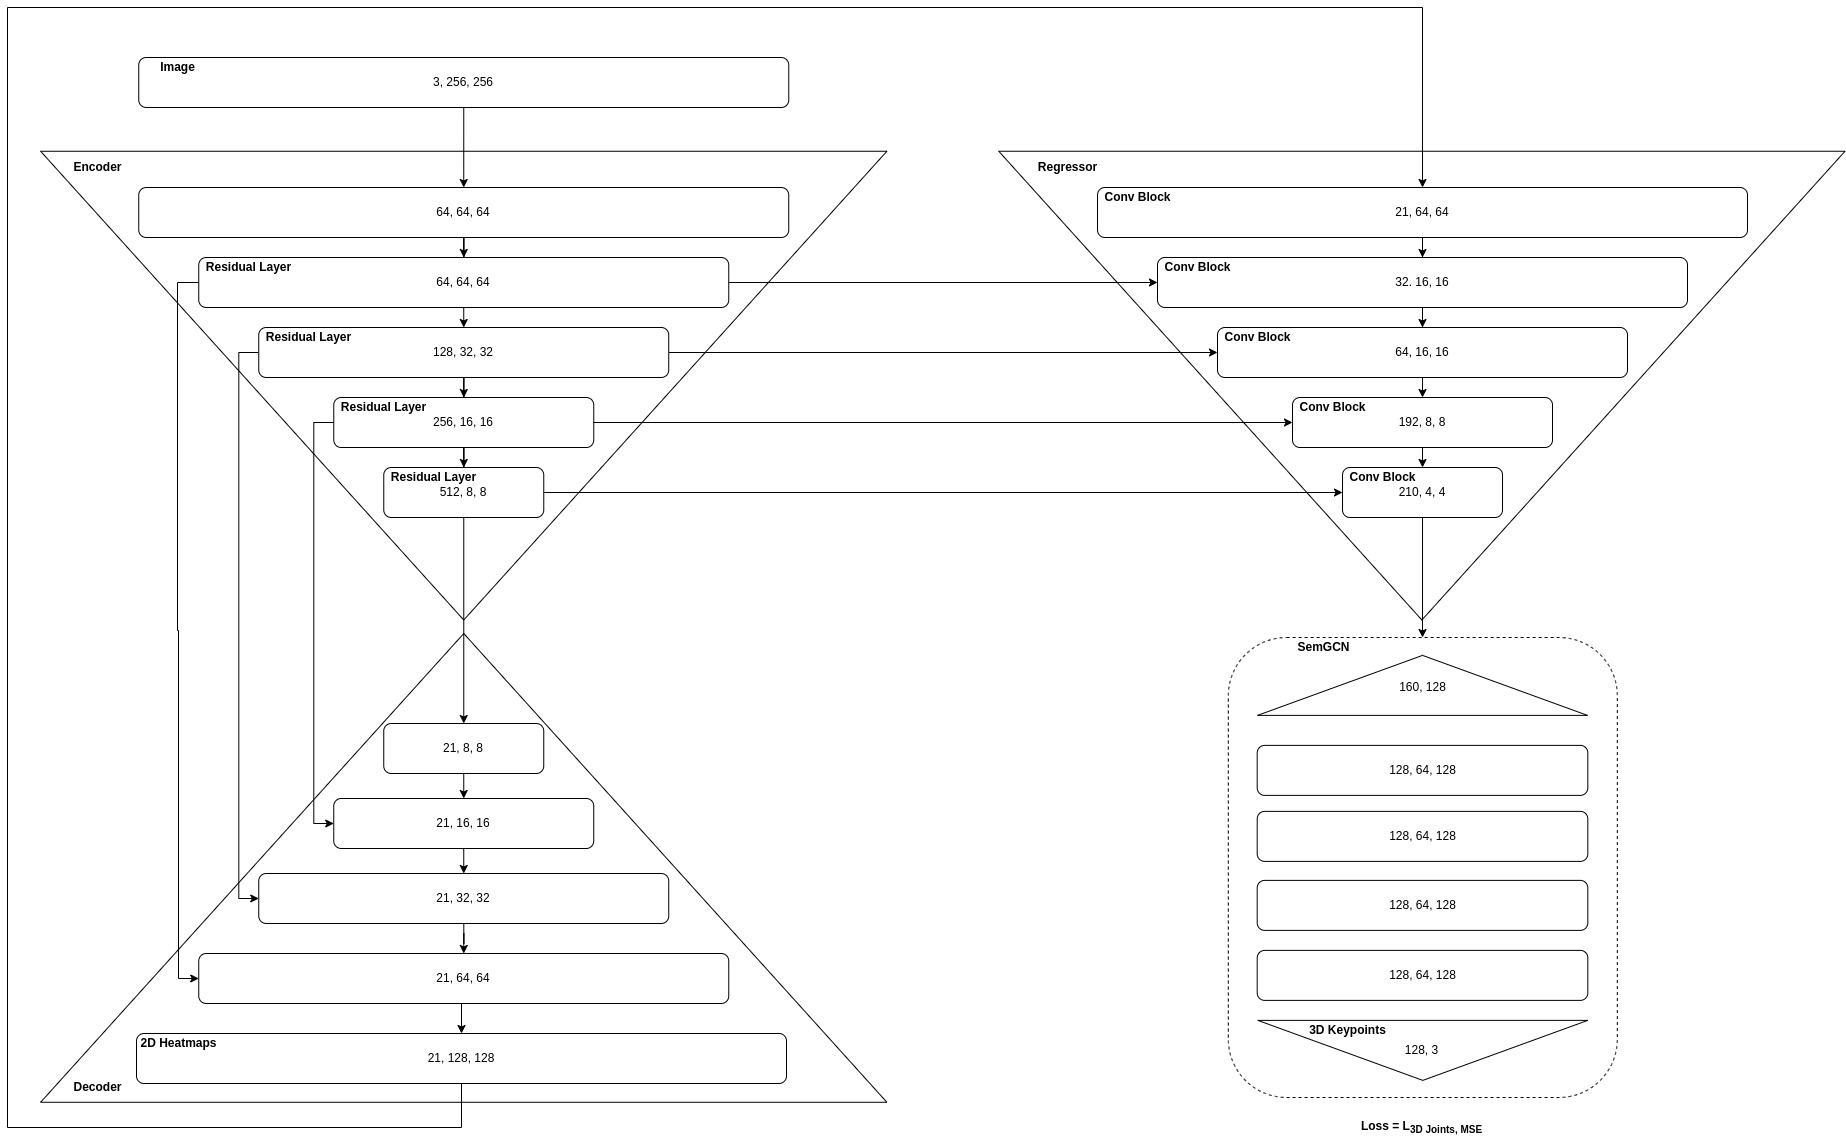
\includegraphics[width=450px]{assets/Model_v4.jpg}
		\caption{Model v4}
		\label{fig:model_v4}
	\end{center}
\end{figure}

\newpage

\noindent
The hyperparameters of the fourth model are modified, keeping the encoder-decoder module the same. Figure \ref{fig:model_v4_x} shows 4 different modifications to Model v4. The top left regressor is the original version. The top right regressor removes the heat map layer, the bottom left regressor increases the number of output channels in each layer, and the bottom right regressor decreases the output channels in each layer. Like the first, second, and third model, the same set hyperparameters were modified in the fourth model to concur the impact on the performance.


\begin{figure}[ht]
	\begin{center}
		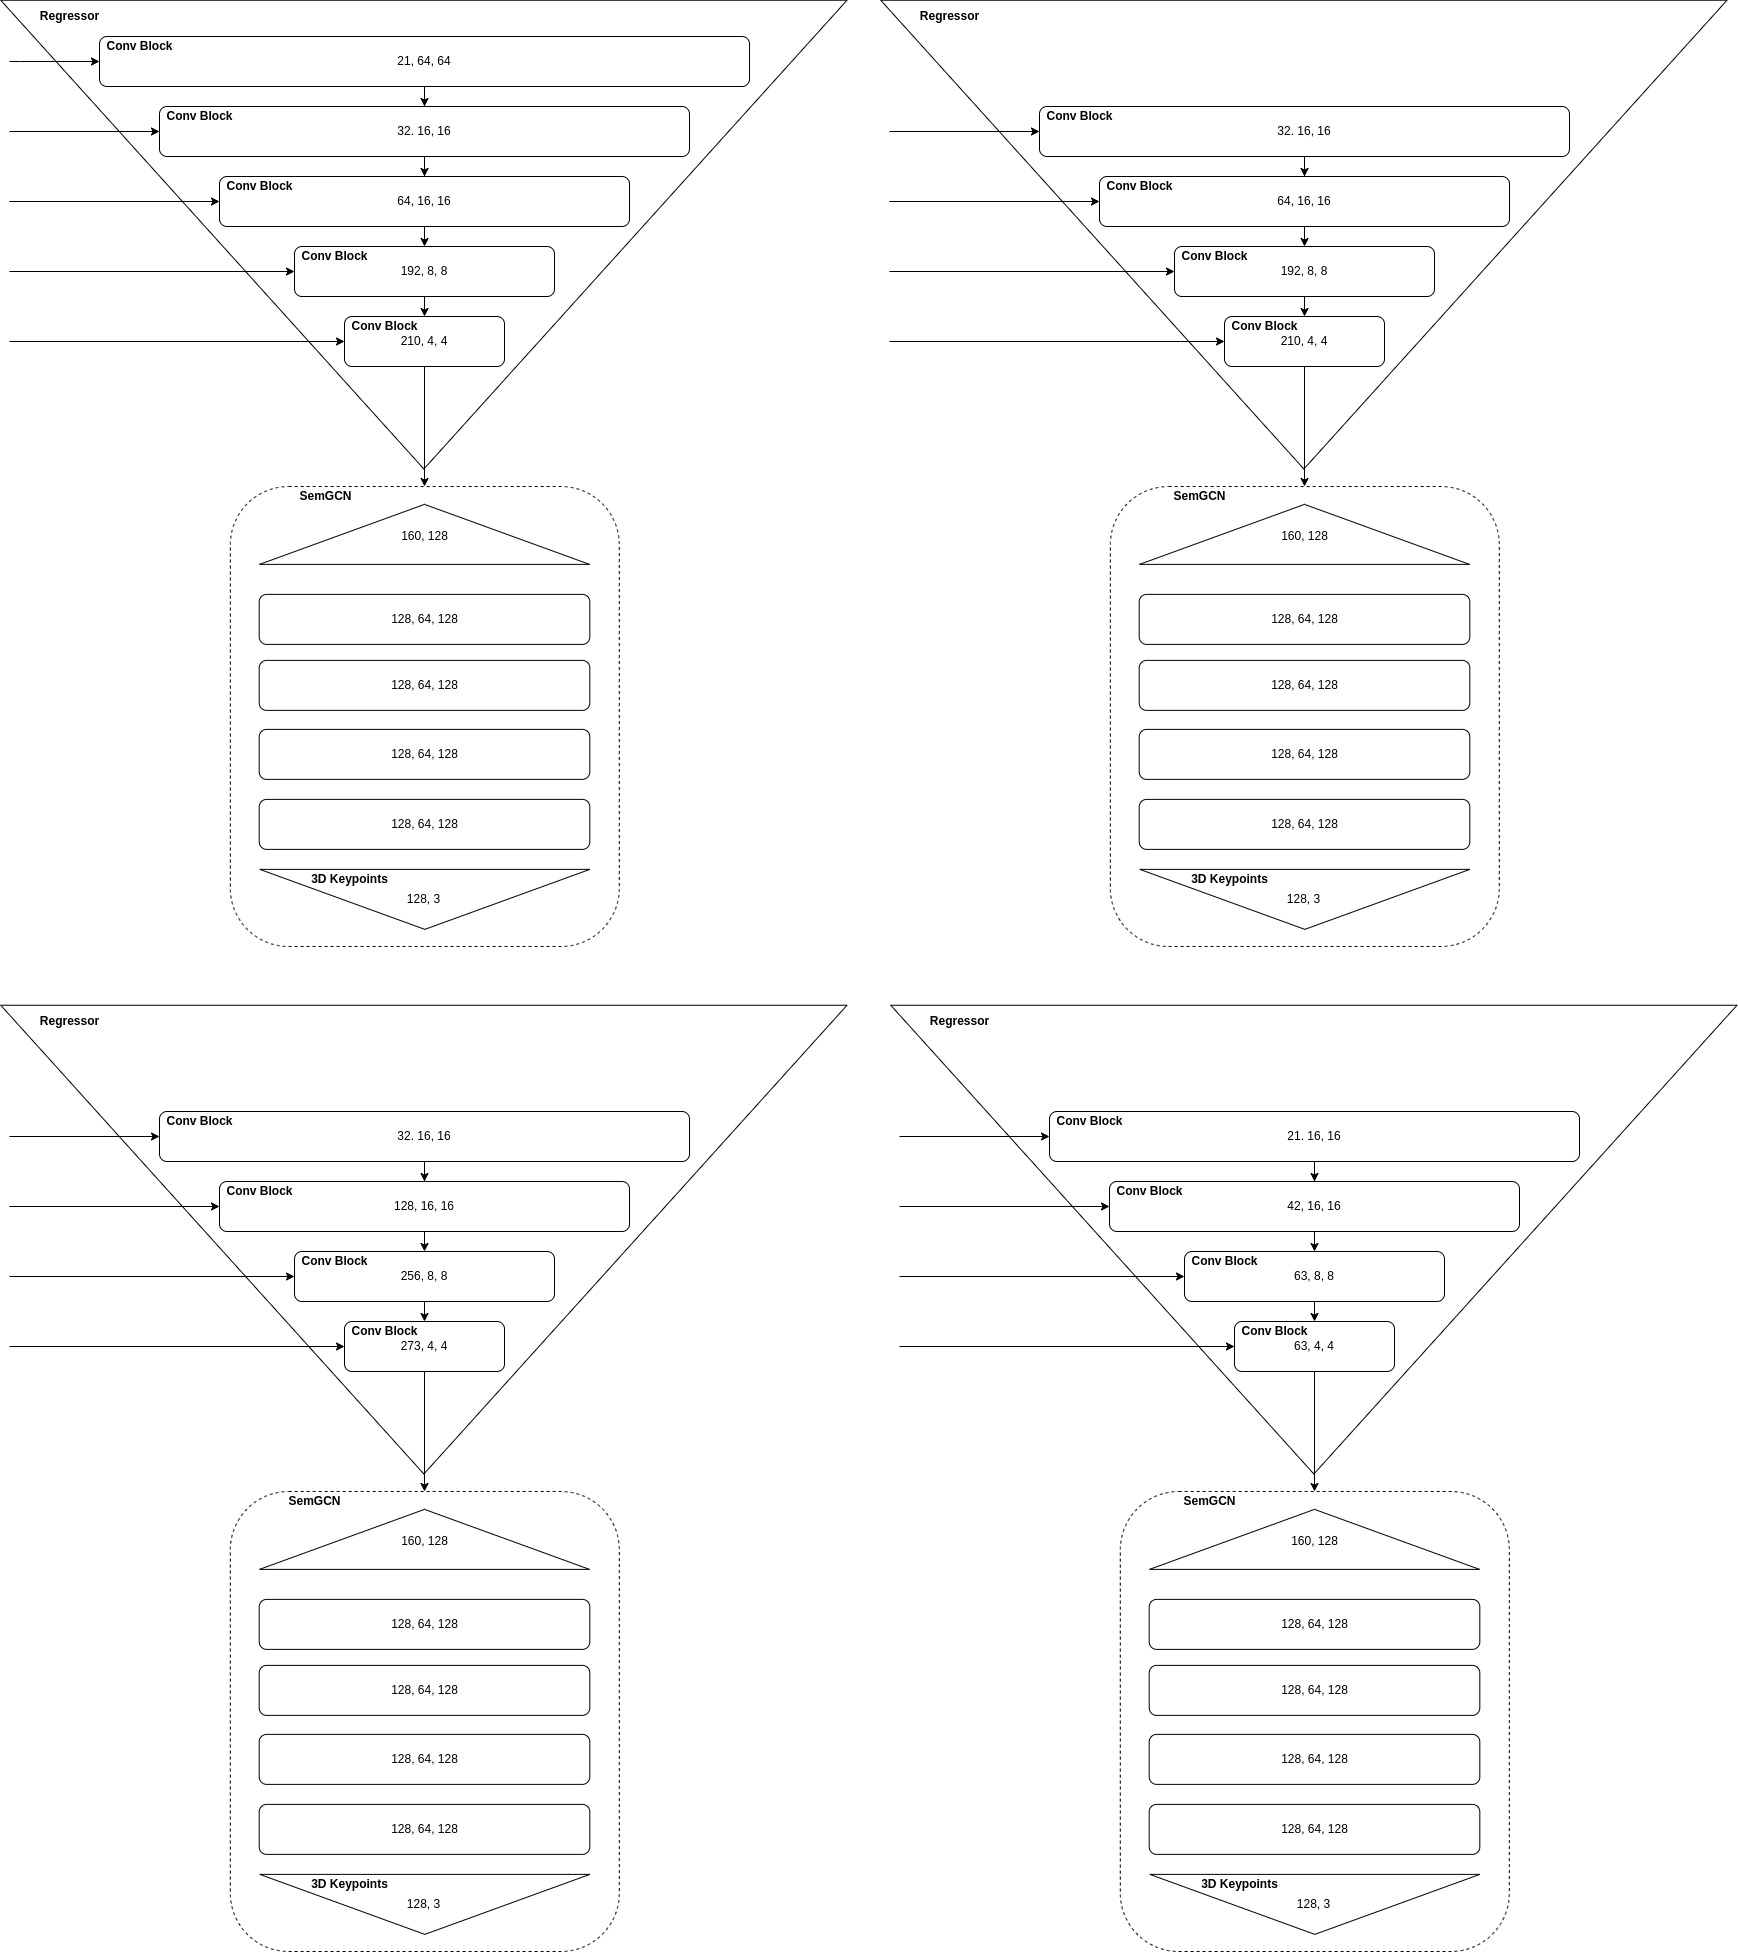
\includegraphics[width=450px]{assets/Model_v4.x.jpg}
		\caption{Hyperparameter Tuning For Model v4}
		\label{fig:model_v4_x}
	\end{center}
\end{figure}

\newpage

\noindent
Later in the results and dicussion, Model v3.1 performed the best and was optimized further. Figure \ref{fig:model_v3_1_x} shows the hyperparameters experimented. The top left regressor used two SemGCN layers and the top middle regressor used 6 SemGCN layers instead of the original 4 layers to understand how the model performs under with more layers and parameters. The top right regressor used two convolution layers instead of one but the output size of the first layer is half of the output size of the second. This reduce the parameters but add depth in the model to determine whether adding layers helps the model learn better than adding channels. The bottom two regressors use additional loss functions. The left regressor is supervised by the MSE of the 2D joints and 3D joints. The right regressor is supervised by the MSE of the 3D joints and 3D bone vector.

\begin{figure}[ht]
	\begin{center}
		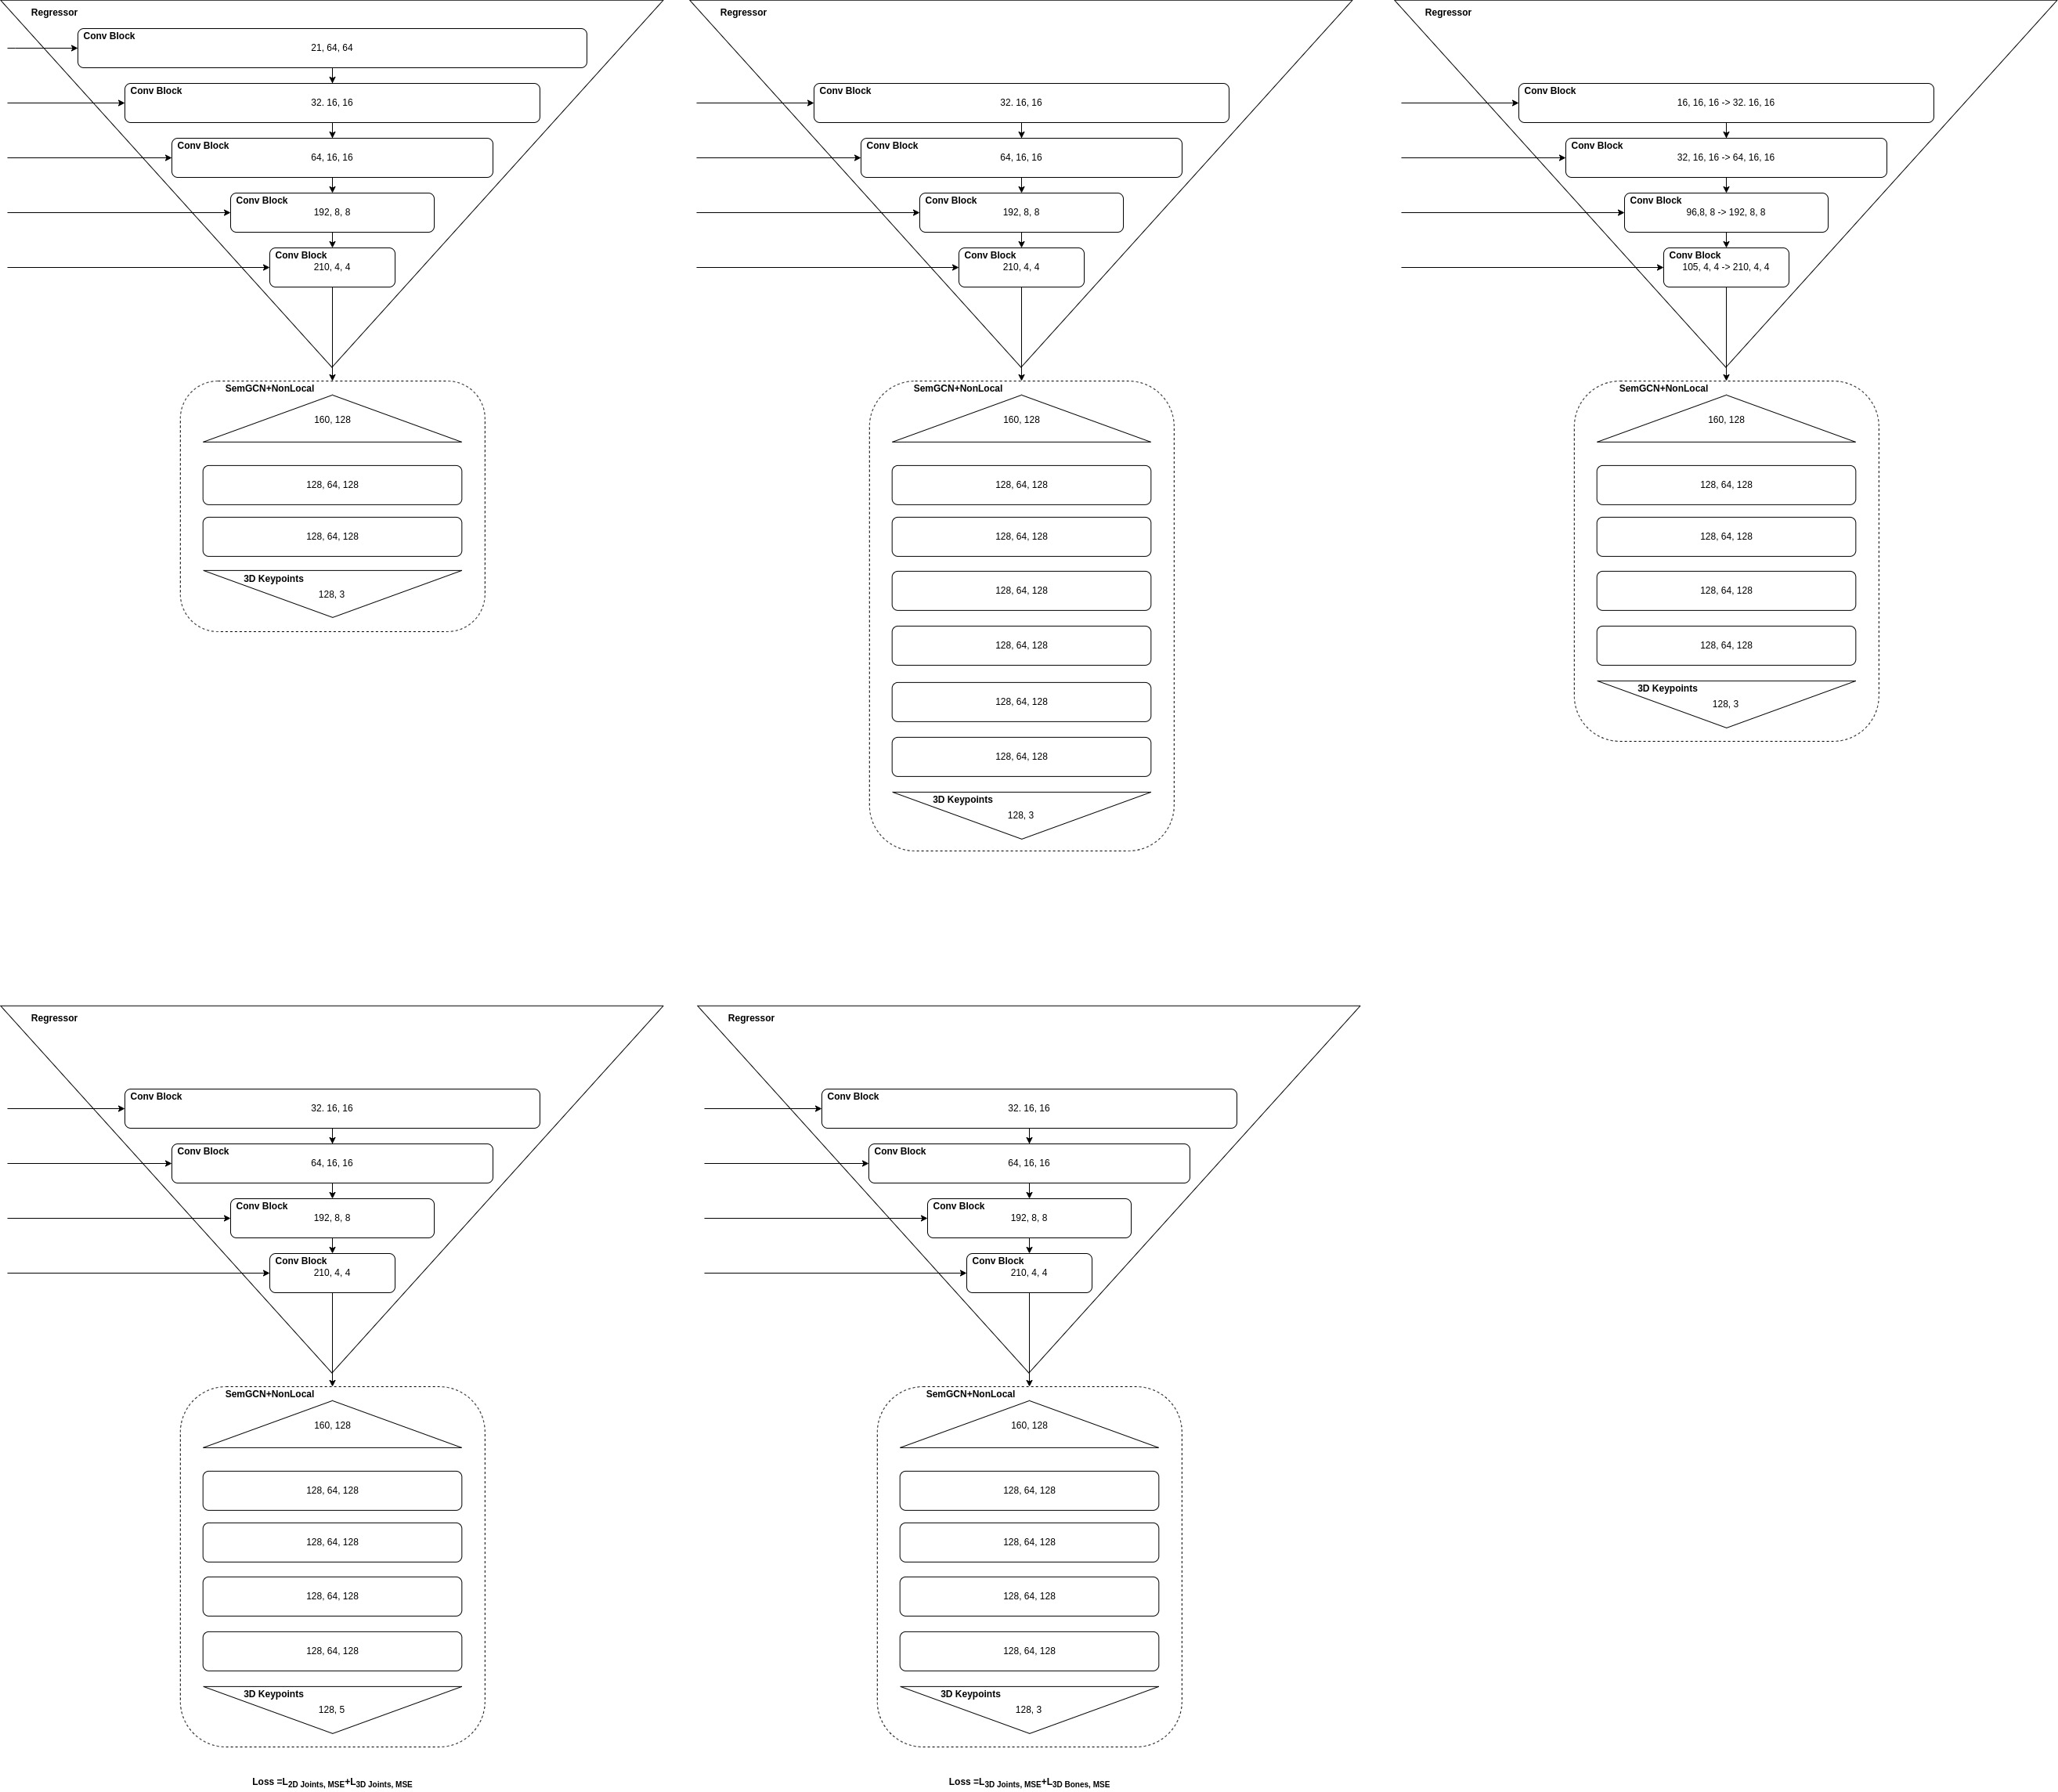
\includegraphics[width=450px]{assets/Model_v3.1.x.jpg}
		\caption{Hyperparameter Tuning For Model v3.1.x}
		\label{fig:model_v3_1_x}
	\end{center}
\end{figure}

\newpage
\noindent
Table \ref{table:model_summary} summarises the different models experimented in this project. The hyperparameters experimented are the heat maps, convolution and regression blocks in the regressor module, SemGCN and fully-connected layer in final layer, and the loss functions. After all the experiments, this project uses v3.1.6 as the final model.

\begin{table}[ht]
\centering
\begin{tabular*}{\textwidth}{c @{\extracolsep{\fill}} cccc}
\hline
Models & Heat map & Regressor Module & Final Layer & MSE Loss Function \\ [0.5ex] 
\hline
v1.0  & Yes & 1 Conv + Residual Block & Fully-Connected & 3D Joints \\
v1.1  & No & 1 Conv + Residual Block & Fully-Connected & 3D Joints \\ 
v1.2  & No & 1 Conv + Residual Block & Fully-Connected & 3D Joints \\ 
v1.3  & No & 1 Conv + Residual Block & Fully-Connected & 3D Joints \\ 
v2.0  & Yes & 1 Conv & Fully-Connected & 3D Joints \\
v2.1  & No & 1 Conv & Fully-Connected & 3D Joints \\ 
v2.2  & No & 1 Conv & Fully-Connected & 3D Joints \\ 
v2.3  & No & 1 Conv & Fully-Connected & 3D Joints \\ 
v3.0  & Yes & 1 Conv & 4 SemGCN + NonLocal & 3D Joints \\
v3.1  & No & 1 Conv & 4 SemGCN + NonLocal & 3D Joints \\ 
v3.2  & No & 1 Conv & 4 SemGCN + NonLocal & 3D Joints \\ 
v3.3  & No & 1 Conv & 4 SemGCN + NonLocal & 3D Joints \\ 
v4.0  & Yes & 1 Conv & 4 SemGCN & 3D Joints \\
v4.1  & No & 1 Conv & 4 SemGCN & 3D Joints \\ 
v4.2  & No & 1 Conv & 4 SemGCN & 3D Joints \\ 
v4.3  & No & 1 Conv & 4 SemGCN & 3D Joints \\ 
v3.1.0  & No & 1 Conv & 4 SemGCN + NonLocal & 3D Joints \\
v3.1.1  & No & 1 Conv & 2 SemGCN + NonLocal & 3D Joints \\
v3.1.2  & No & 1 Conv & 6 SemGCN + NonLocal & 3D Joints \\
v3.1.3  & No & 2 Conv & 4 SemGCN + NonLocal & 3D Joints \\
v3.1.4  & No & 1 Conv & 4 SemGCN + NonLocal & 2D Joints + 3D Joints \\
v3.1.5  & No & 1 Conv & 4 SemGCN + NonLocal & 3D Joints + 3D Bone \\
v3.1.6  & No & 2 Conv & 4 SemGCN + NonLocal & 3D Joints + 3D Bone \\
[1ex] 
\hline
\end{tabular*}
\caption{Model summary}
\label{table:model_summary}
\end{table}

\newpage


\subsection{Training Details}
\noindent
The training details are for the Pose 2D Estimator and Pose 3D Regressor are described in Table \ref{table:training_details}. The Pose 2D Estimator is first trained without the Pose 3D Regressor and is supervised by the IoU loss function. The encoded features from the Pose 2D Estimator serves as the image embedding for the Pose 3D Regressor and is supervised by the MSE loss functions of the joint positions and bone vectors.

\begin{table}[ht]
\centering
\begin{tabular*}{\textwidth}{c @{\extracolsep{\fill}} p{4.5in} p{0.0in}}
\hline
Training Detail & \centering Description & {} \\ [0.5ex] 
\hline
Epochs  & Trained for about 200 epochs for Pose 2D and 50 epochs for Pose 3D till the validation loss saturated & {} \\
Batch Size  & Trained using minibatch size of 32 to average the loss & {} \\ 
Optimizer  & Trained with Adam optimizer to adapt the learning rate for different parameters & {} \\ 
Learning Rate  & Trained with 0.001 for the first half epochs and 0.0001 for the second half to fine tune performance  & {}\\ 
Embedding  & Trained 3D Regressor using the encoded features in Pose 2D Rstimator as image embedding & {}\\ 
Workers  & Set workers to 8 to reduce time spent in I/O computation & {}\\ 
Shuffle  & Set shuffle flag to true when training the model to vary the training data & {}\\ 
Loss Function  & Supervisor training for Pose 2D Estimator using IoU loss and Pose 3D Regressor using MSE & {}\\ 
[1ex] 
\hline
\end{tabular*}
\caption{Training Details}
\label{table:training_details}
\end{table}
\noindent
Figure \ref{fig:hand_annnotation} shows the annotation of 2D heat maps (left) and 3D poses (right) of the hand. The bright spots in the 2D heat maps indicates where the keypoints in the image are. Guassian blur is applied on the bright spot to prevent the model from overfitting. The 3D pose is centered with the middle knuckle/middle 1 (refer to Appendix B) at the origin. The length of the hand is measured in meters to keep the range of the values from -1 to 1. The same annotation method is applied for the upper body pose with the spine centered at the origin (refer to Appendix A).
\begin{figure}[ht]
    \begin{center}
        \begin{subfigure}[b]{0.5\textwidth}
            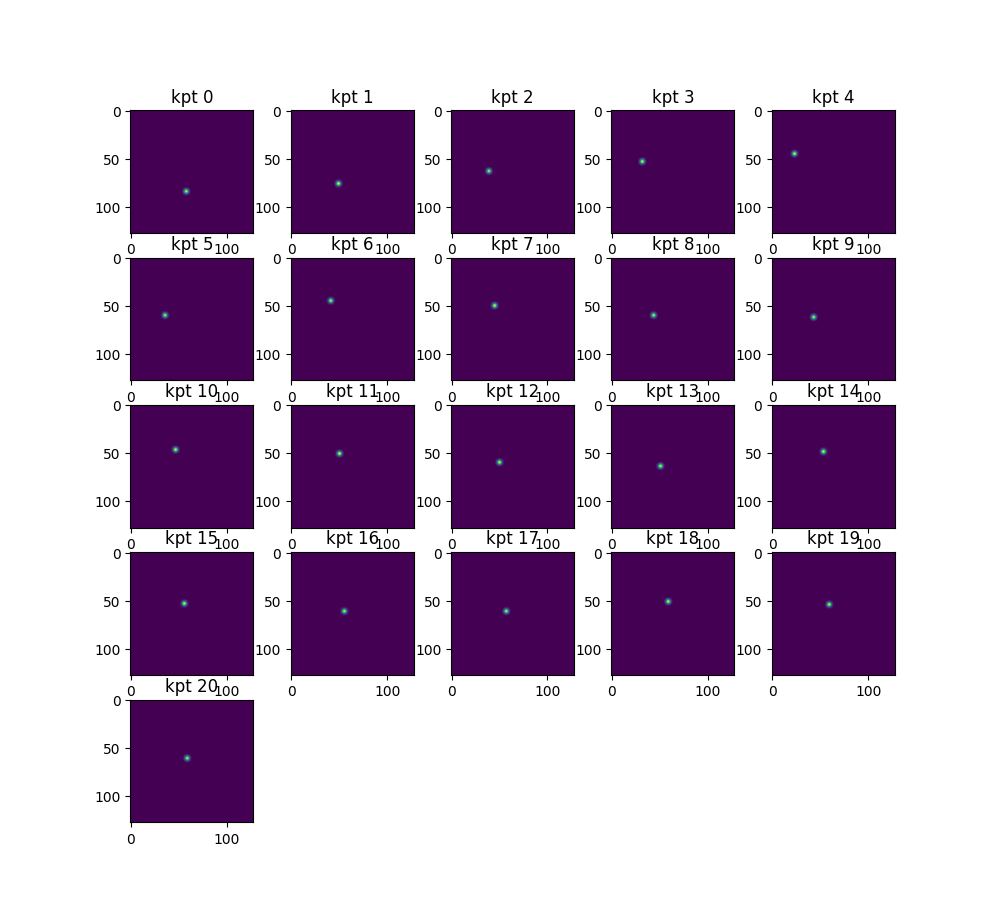
\includegraphics[width=250px]{assets/hand_heatmap_annotation.png}
            \caption{Pose 2D}
            \label{fig:hand_heatmap_annotation}
        \end{subfigure}
        \begin{subfigure}[b]{0.45\textwidth}
            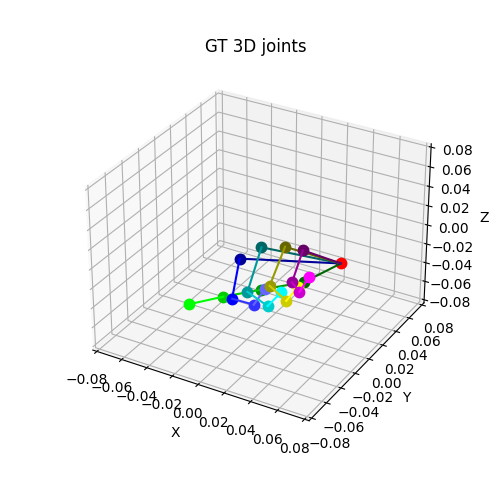
\includegraphics[width=200px]{assets/hand_pose_annotation.png}
            \caption{Pose 3D}
            \label{fig:hand_pose_annotation}
        \end{subfigure}
	    \caption{Pose Annotation}
	    \label{fig:hand_annnotation}        
    \end{center}
\end{figure}

\noindent
The IoU loss function is applied on the predicted heat maps to supervise the Pose 2D Estimator to learn the ground truth 2D heat maps \cite{olha}. The equation to compute the IoU loss is given in Equation \ref{eq:chernytska_iou_loss} \cite{olha}. The IoU measures the overlaps between the heatmaps for continuous values as shown in Equation \ref{eq:chernytska_iou}. The IoU loss is a value in the range from 0 to 1. A value close to 1 means the predicted matches the ground truth heatmaps and vice-versa. False negative is penalized in the Equation \ref{eq:chernytska_iou_intersection}, while false positive is penalized in the second term of Equation \ref{eq:chernytska_iou_union}.
\begin{equation}
L_{IoU} = 1 - IoU \label{eq:chernytska_iou_loss}
\end{equation}
\begin{equation}
IoU = \frac{I}{U} \label{eq:chernytska_iou}
\end{equation}
\begin{equation}
I = \sum_{i} (y_{pred,i} * y_{true,i}) \label{eq:chernytska_iou_intersection}
\end{equation}
\begin{equation}
U = \sum_{i} (y_{pred,i} * y_{pred,i}) + \sum_{i} (y_{true,i} * y_{true,i}) - \sum_{i} (y_{pred,i} * y_{true,i}) \label{eq:chernytska_iou_union}
\end{equation}
\noindent
The MSE loss function is applied on the predicted 3D poses to supervise the Pose 3D Regressor to learn the ground truth 3D poses \cite{semgcn, poseestimationreview}. The equation to compute the MSE loss is given in Equation \ref{eq:joint_positions_mse} \cite{semgcn, poseestimationreview}. The model treats the 3D poses as a regression tasks. A small loss indicates the predicted 3D poses matches the ground truth.
\begin{equation}
L_{mse} = \sum_{i} (P_{pred,i} - P_{true,i})^{2}\label{eq:joint_positions_mse}
\end{equation}
\noindent
The MSE loss function can also be applied on the predicted 3D bone vector to supervise the Pose 3D Regressor to learn the ground truth 3D bone vector \cite{semgcn}. The bone vector is computed by subtracting the positions of two 3D keypoints. The bone vector provides information on the direction and bone length that can help the model learn better. The equation to compute the MSE loss is given in Equation \ref{eq:bone_vector_mse} \cite{semgcn}. A small loss indicates the predicted 3D bone vectors matches the ground truth.
\begin{equation}
L_{mse} = \sum_{i} (B_{pred,i} - B_{true,i})^{2}\label{eq:bone_vector_mse}
\end{equation}


\newpage
\subsection{Robotic Arm Setup}
\noindent
MyCobot is setup to teleoperate via gestures from pose estimation on RGB images. Figure \ref{fig:robotic_arm_setup} shows the setup of the robotic arm in simulation on the left and in the real world on the right \cite{mycobot}. Unity3D is used for simulation \cite{unity3d}. The URDF of MyCobot is modified to include the gripper.

\begin{figure}[ht]
    \begin{center}
        \begin{subfigure}[b]{0.40\textwidth}
            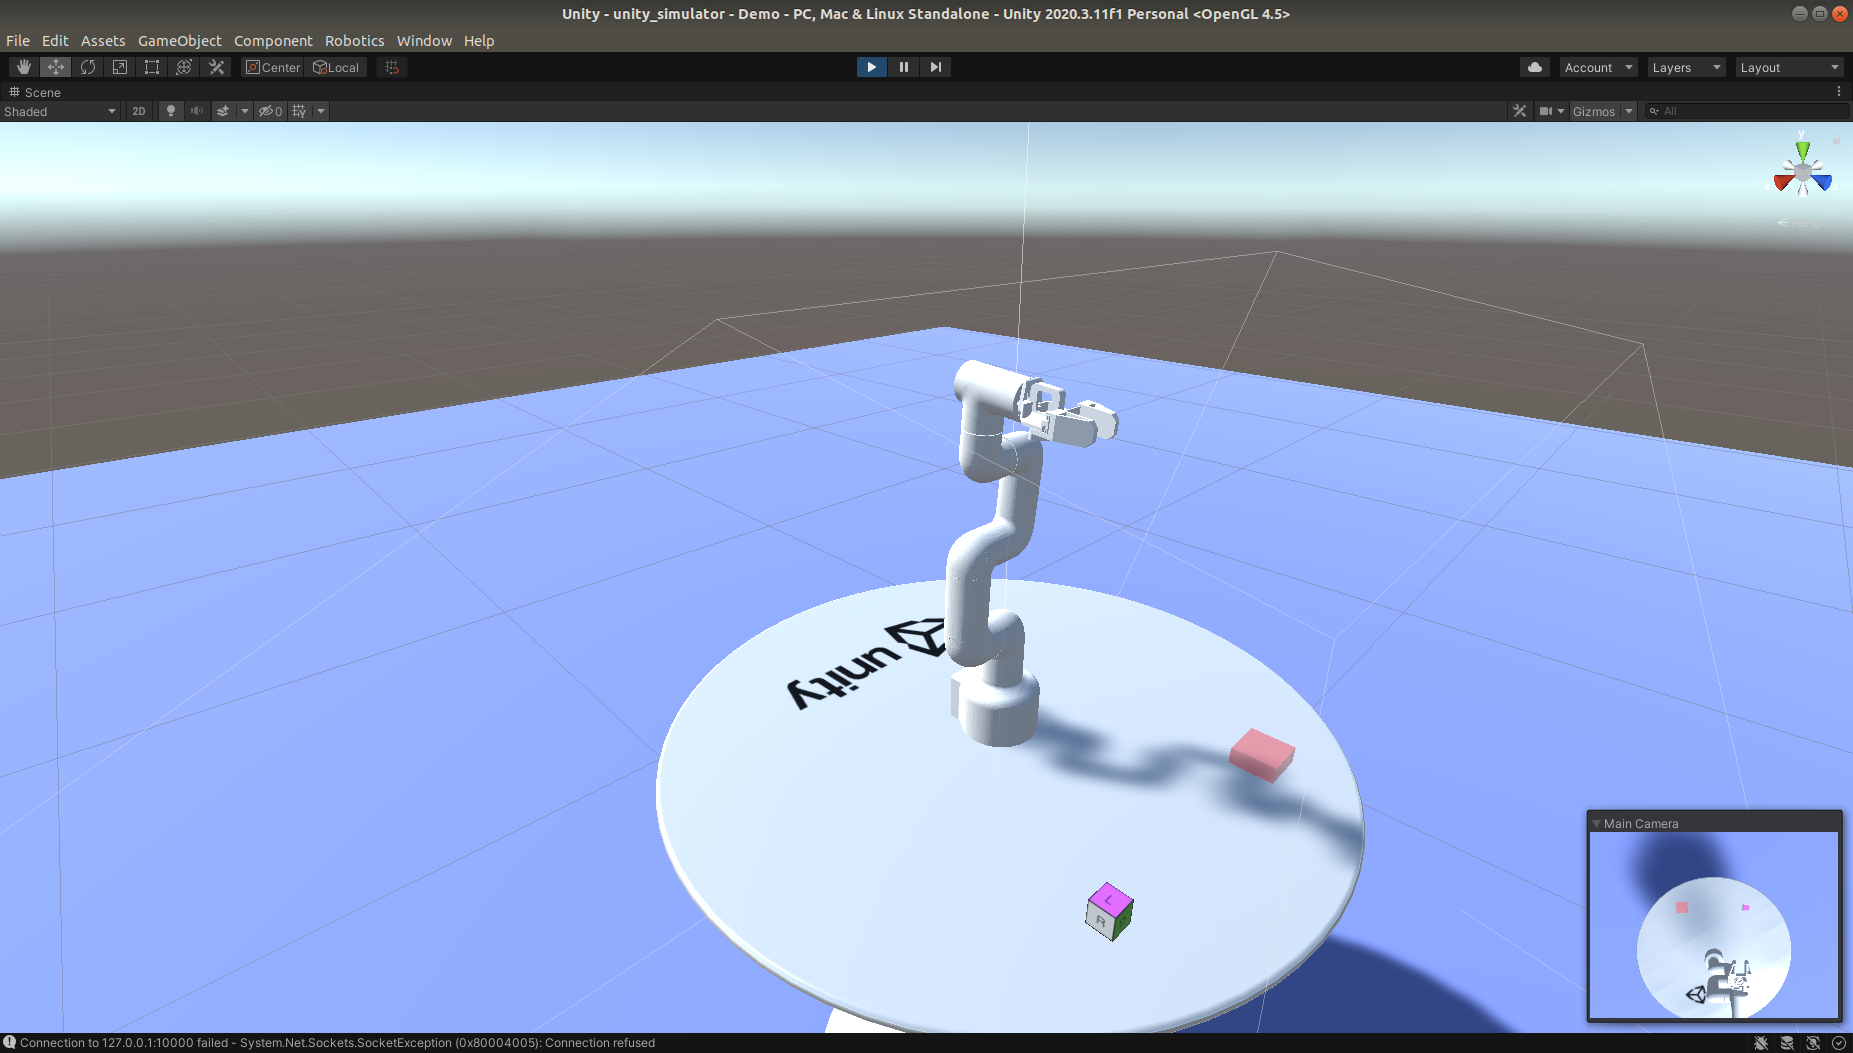
\includegraphics[width=180px]{assets/simulation_robot.png}
            \caption{Simulated Robot}
            \label{fig:simulated_robot}
        \end{subfigure}
        \begin{subfigure}[b]{0.22\textwidth}
            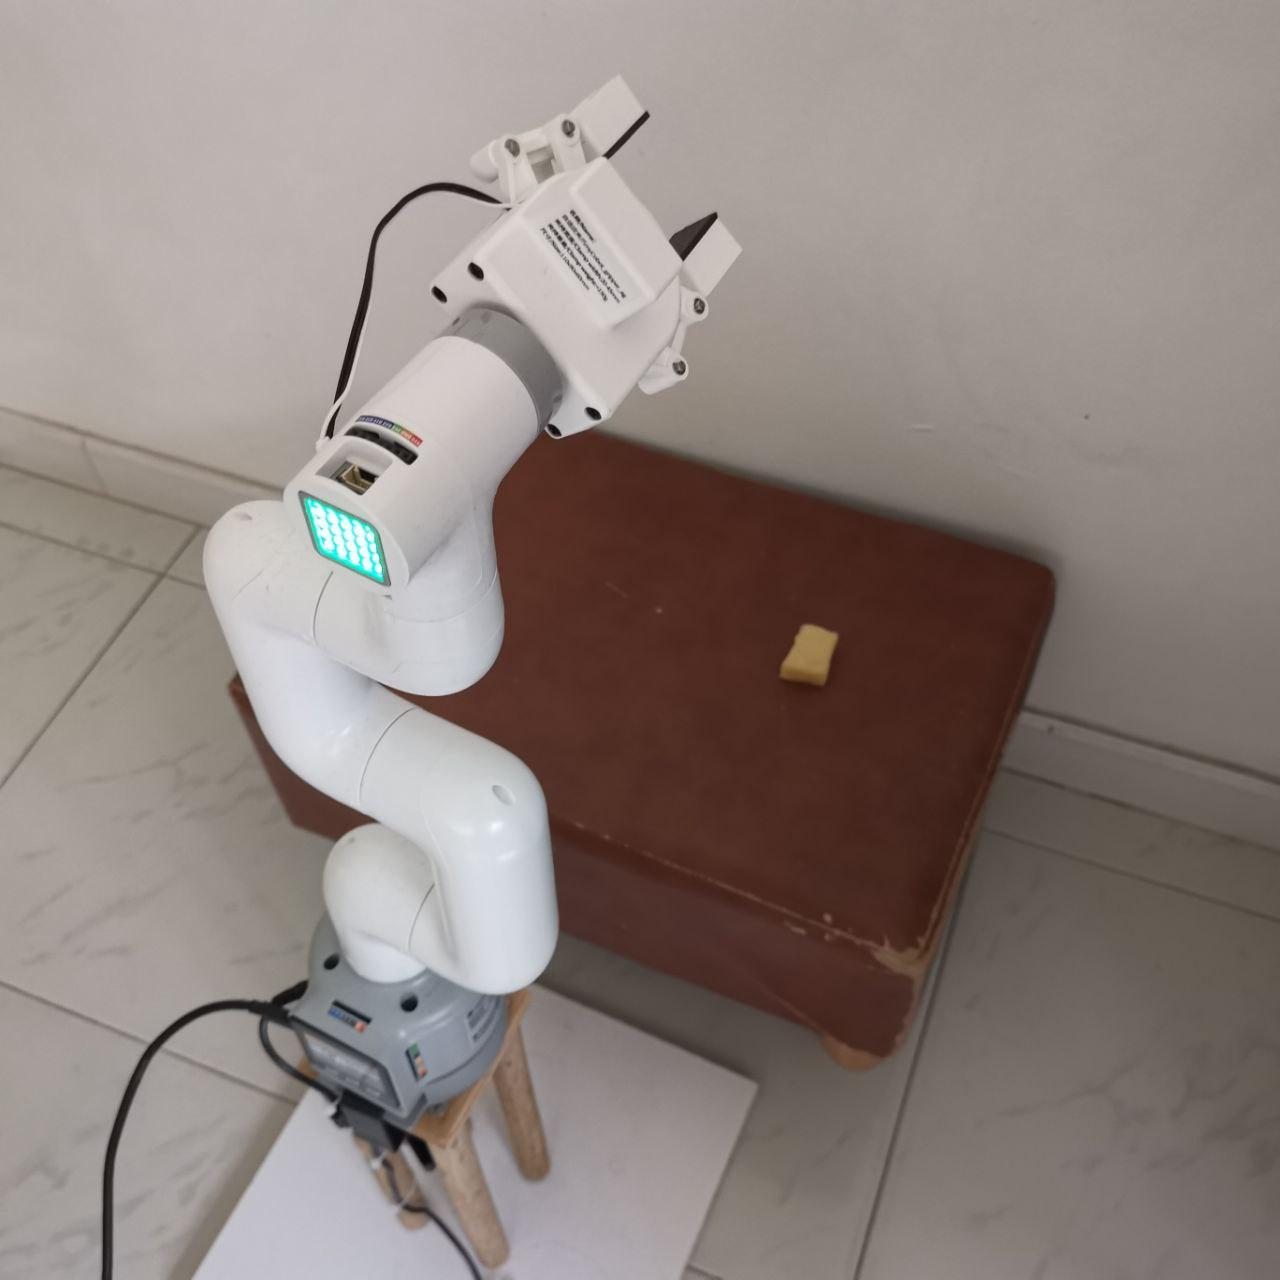
\includegraphics[width=100px]{assets/physical_robot.jpg}
            \caption{Physical Robot}
            \label{fig:physical_robot}
        \end{subfigure}
	    \caption{Robotic Arm Setup}
	    \label{fig:robotic_arm_setup}        
    \end{center}
\end{figure}
\noindent
ROS is used to modularise the robot development into subsystems, namely perception, navigation, and controller, as shown in Figure \ref{fig:ros_setup}. The Pose node extracts 3D poses from RGB images and publishes the pose. The Joints node publishes the current robot joints. The Controller node subscribes and receives the current robot joints and 3D poses. The Controller node also computes the start pose and end pose. The Trajectory Planner Service node plans the trajectory from start to end pose, while the Robot Motion Action Server node executes the trajectory to move the real robot and simulated robot.

\begin{figure}[ht]
	\begin{center}
		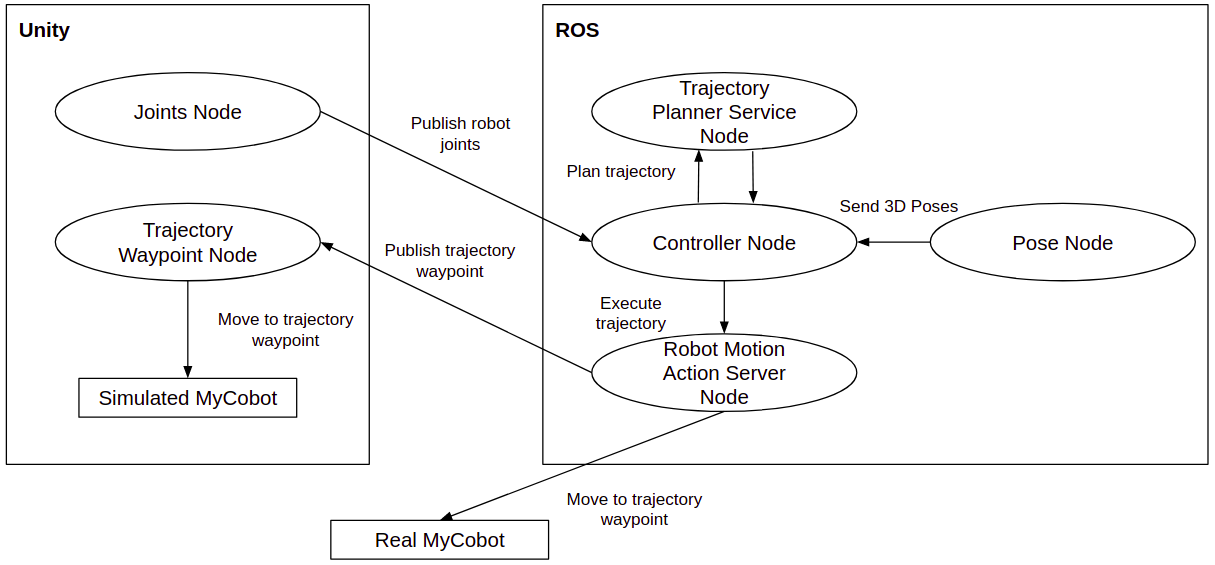
\includegraphics[width=300px]{assets/ros_setup.png}
		\caption{ROS Setup}
		\label{fig:ros_setup}
	\end{center}
\end{figure}


\newpage
\section{Results And Discussion}

\subsection{Metrics}
\noindent
The Mean Per Joint Position Error (MPJPE) is a metric to determine the euclidean distance between the predicted and ground truth 3D poses. This is a common metric used in papers for 3D Pose Estimation \cite{poseestimationreview}. The MPJPE is also computed per keypoint to understand the error distribution. Equation \ref{eq:mpjpe} shows how the euclidean distance error is computed.
\begin{equation}
E = \sum_{i=1} |\mathbf{p_{pred}} (i) - \mathbf{p_{gt}} (i)| \label{eq:mpjpe}
\end{equation}
\noindent
The Percentage of Correct Keypoints (PCK) is a metric to determine if the keypoints are predicted correctly if they fall within the radius of the ground truth keypoints. In this project, PCK@5mm and PCK@15mm are used to evaluate the percentage of correct keypoints if they are 5mm or 15mm within the grouth truth. This metric is easy to understand in terms of measuring accuracy. PCK@5mm is stricter than PCK15mm to measure the precision of keypoints. Equation \ref{eq:pck} shows how the PCK@5mm and PCK@15mm error is computed.
\begin{equation}
Accuracy_{<5/15mm} = \frac{N_{keypoints<5/15mm}}{N_{keypoints}} \times 100\% \label{eq:pck}
\end{equation}

\newpage
\subsection{Hand Pose Evaluation}
\noindent
The models were trained and evaluated using the metrics MPJPE, PCK@5mm and PCK@15mm. Table \ref{table:model_evaluation_hand_pose} shows the performance of the models trained for different architectures - residual blocks, graph convolution layers, and non-local layers. Table \ref{table:model_evaluation_hand_pose} also shows the models trained for different hyperparameters - heat maps, more channels, and fewer channels. Refer to Table \ref{table:model_summary} for exact differences of the model architectures.

\begin{table}[ht]
\centering
\begin{tabular*}{\textwidth}{c @{\extracolsep{\fill}} ccccc}
\hline
Model & Params & FPS & MPJPE & PCK@5mm & PCK@15mm \\
\hline
v1.0 & 13.44M & 12.6 & 8.66 & 30.77 & 87.85 \\ 
v1.1 & 13.30M & 14.77 & 8.24 & 34.68 & 89.04 \\
v1.2 & 16.85M & 13.85 & 8.64 & 32.05 & 87.46 \\
v1.3 & 8.58M & 17.33 & 9.24 & 29.99 & 84.63 \\
v2.0 & 2.08M & 20.16 & 10.61 & 21.73 & 80.08 \\ 
v2.1 & 2.07M & 21.02 & 10.46 & 22.95 & 80.14 \\
v2.2 & 8.20M & 18.14 & 11.84 & 17.24 & 74.90 \\
v2.3 & 0.63M & 22.47 & 12.47 & 17.02 & 70.57 \\
v3.0 & 2.19M & 18.02 & 8.24 & 35.63 & 88.76 \\ 
v3.1 & 2.18M & 19.17 & 8.28 & 33.84 & 89.41 \\
v3.2 & 8.46M & 16.23 & 7.64 & 39.70 & 90.70 \\
v3.3 & 0.72M & 19.40 & 9.10 & 33.65 & 84.90 \\
v4.0 & 2.18M & 18.99 & 8.31 & 34.71 & 88.89 \\ 
v4.1 & 2.17M & 20.00 & 8.63 & 33.26 & 87.76 \\
v4.2 & 8.45M & 17.38 & 8.09 & 37.64 & 88.89 \\
v4.3 & 0.71M & 21.01 & 10.25 & 24.60 & 81.43 \\
[1ex] 
\hline
\end{tabular*}

\caption{Model Evaluation For Hand Pose}
\label{table:model_evaluation_hand_pose}
\end{table}

\noindent
Models v1.X uses 1 convolution layer and 1 residual block for each layer of the 3D Regressor module and generally has low MPJPE error and high PCK accuracy as compared to the other models. However, the number of trainable parameters is almost 7 times more than their counterparts. The residual blocks contributed to most of the paramters. Out of the 4 different hyparameters tested for v1.X, v1.1 that was trained without the heat maps performed the best. v1.2 was trained with more channels but did not show improvements, and v1.3 was traiend with fewer channels and showed worst performance.

\noindent
Models v2.X uses 1 convolution layers for each layer of the 3D Regressor module and did not perform as well as v1.X. The residual block added complexity to the model and allowed it to learn and estimate the 3D poses better. Similar to v1.1, v2.1 also demonstrates the heat maps did not contribute to any improvement in the model performance. v2.2 and v2.3 also similarly show more and fewer channels did not improve the model performance.

\noindent
Models 3.X uses graph convolution layers (SemGCN) and non-local layers instead of the fully-connected layer as the final layer in the 3D Regressor module. v3.1 similarly demonstrates the heat maps did not improve the model performance. v3.3 has fewer channels and performed poorly. Interestingly, v3.2 that was trained with more parameters performed the best out of all the models in this table. The graph convolution layers and non-local layers were able to learn better with more features from the convolution layers.

\noindent
Models 4.X uses graph convolution layers (SemGCN), but unlike 3.X, these models do not have the non-local layers. v4.1 similarly demonstrates the heat maps did not improve the model performance. v4.3 has fewer channels and performed poorly. v4.2 does not perform as well as v3.2. This strongly suggests the non-local layers in v3.2 learn the long distance relationship between entities in the graph, contributing to better 3D pose estimations.

\noindent
Using the results of Table \ref{table:model_summary}, it is evident that Model v3.2 performs the best. However, v3.2 has 4 times more parameters than v3.1. v3.1 still performs reasonably well with fewer paramters. Table \ref{table:model_evaluation_fc} shows the second round of hyperparameters tuning for Model v3.1 to push the model performance further. v3.1.0 has the same architecture as v3.1.0 but the v3.1.0 was further trained end-to-end without freezing the encoder-decoder layers. Models v3.1.x were similarly trained end-to-end, after training the 3D Regressor module alone with the encoder layers freezed.

\begin{table}[ht!]
\centering
\begin{tabular*}{\textwidth}{c @{\extracolsep{\fill}} ccccc}
\hline
Model & Params & FPS & MPJPE & PCK@5mm & PCK@15mm \\
\hline
v3.1.0 & 2.18M & 19.17 & 7.29 & 40.78 & 92.78 \\
v3.1.1 & 2.11M & 20.05 & 7.32 & 41.59 & 92.49 \\
v3.1.2 & 2.24M & 18.38 & 6.93 & 44.52 & 93.64 \\
v3.1.3 & 1.57M & 19.37 & 6.87 & 44.94 & 93.89 \\
v3.1.4 & 2.18M & 19.13 & 8.52 & 30.43 & 89.30 \\
v3.1.5 & 2.18M & 19.17 & 6.87 & 45.27 & 93.56 \\
[1ex] 
\hline
\end{tabular*}
\caption{Model Evaluation (Variations Of v3.1.X)}
\label{table:model_evaluation_fc}
\end{table}

\noindent
v3.1.0 shows that the model did better after further training end-to-end. v3.1.1 shows the model did not perform as well as v3.1.0 after using 2 graph convolution and non-local layers instead of 4. v3.1.2 showed the model performed better using 6 graph convolution and non-local layers instead of 4, although the number of trainable parameters increased by 0.13M. v3.1.3 added 1 more convolution layer at each layer of the 3D Regressor module where the number of output channels of first convolution is half of the number of output channels second convolution layer. This adds depth to model while reducing the number of parameters. Interestingly, the model was able to perform better. v3.1.4 was trained using two loss functions, mean squared error of the 2D poses and mean squared error of the 3D poses. However, the model does not show improvements. v3.1.5 was trained using two loss functions too, mean squared error of the 3D poses and mean squared error of the 3D bone vector. The bone vector encoder the orientation of two joints to correct the direction of the joint positions. The model showed improvements with a higher PCK@5mm.

\begin{table}[ht!]
\centering
\begin{tabular*}{\textwidth}{c @{\extracolsep{\fill}} cccccc}
\hline
Model & Dataset & Full Params & Pose 3D Module Params & MPJPE \\
\hline
Ours & NTU & 23.05M & 1.57M & \(6.79^{*}\) \\ 
L. Ge \cite{handgcn} & NTU & 21.77M & 9.19M & 8.03 \\
Ours & Freihand & 23.05M & 1.57M & \(9.08^{*}\) \\ 
K. Lin \cite{meshgraphormer} & Freihand & 98.43M & - & 6.00 \\
H. Choi \cite{pose2mesh} & Freihand & 74.96M & 67.60M & 7.40 \\ 
[1ex] 
\hline
\end{tabular*}
\caption{Model Evaluation (Benchmark)}
\label{table:model_evaluation_paper_comparison}
\end{table}


\begin{table}[ht!]
\centering
\begin{tabular*}{\textwidth}{c @{\extracolsep{\fill}} cccccc}
\toprule
Model &  \multicolumn{3}{c}{FreiHand} & \multicolumn{3}{c}{NTU} \\[0.5ex] 
\midrule
{} & MPJPE & PCK@5mm & PCK@15mm & MPJPE & PCK@5mm & PCK@15mm \\ 
\hline
Wrist & 9.35 & 18.51 & 88.64 & 6.75 & 44.92 & 96.23 \\ 
Thumb 1 & 8.66 & 20.92 & 91.35 & 5.15 & 64.34 & 97.35 \\
Thumb 2 & 9.56 & 17.25 & 87.43 & 6.10 & 46.15 & 96.80 \\
Thumb 3 & 11.29 & 13.47 & 78.26 & 8.26 & 28.19 & 92.69 \\
Thumb 4 & 16.10 & 6.49 & 58.30 & 10.22 & 20.77 & 86.54 \\ 
Index 1 & 3.88 & 78.09 & 99.37 & 2.65 & 94.91 & 99.23 \\
Index 2 & 6.49 & 42.52 & 96.00 & 6.30 & 55.41 & 93.86 \\
Index 3 & 9.19 & 22.02 & 88.58 & 8.17 & 40.59 & 90.86 \\
Index 4 & 13.64 & 10.08 & 68.89 & 10.76 & 26.61 & 85.36 \\ 
Middle 1 & 1.41 & 100.0 & 100.0 & 1.02 & 99.48 & 100.0 \\
Middle 2 & 5.34 & 54.55 & 98.44 & 5.91 & 56.82 & 95.35 \\
Middle 3 & 9.08 & 21.00 & 89.35 & 7.96 & 39.14 & 91.63 \\
Middle 4 & 14.00 & 8.46 & 68.54 & 10.18 & 26.52 & 86.19 \\ 
Ring 1 & 3.95 & 76.12 & 99.37 & 2.36 & 96.26 & 98.96 \\
Ring 2 & 5.79 & 48.47 & 97.75 & 5.57 & 59.70 & 95.79 \\
Ring 3 & 9.15 & 22.34 & 88.42 & 7.67 & 41.61 & 91.71 \\
Ring 4 & 13.95 & 9.58 & 68.46 & 10.04 & 24.86 & 86.34 \\
Pinky 1 & 6.44 & 39.65 & 97.75 & 4.14 & 78.41 & 98.09 \\
Pinky 2 & 8.12 & 27.25 & 92.72 & 5.96 & 56.47 & 95.30 \\
Pinky 3 & 10.60 & 17.00 & 81.98 & 7.66 & 42.09 & 91.26 \\
Pinky 4 & 14.70 & 8.19 & 64.46 & 9.80 & 29.19 & 85.70 \\
Average & 9.08 & 31.52 & 85.91 & 6.79 & 51.07 & 93.11 \\
[1ex] 
\hline
\end{tabular*}
\caption{Model Evaluation For Keypoints}
\label{table:model_evaluation_keypoints}
\end{table}

\noindent
v3.1.3 shows the model can perform better by adding depth and reducing the trainable parameters. v3.1.5 shows the model can perform better by adding one more loss function. For the final model, the model architecture in v3.1.3 was used and trained using the two loss functions in v3.1.5. The resulting performance is 6.79mm MPJPE on the NTU dataset and 9.08mm MPJPE on the Freihand dataset. Table \ref{table:model_evaluation_paper_comparison} shows our model performance bench-marked against other papers. Note that the asterisk on our model indicates that our model is evaluated differently on the dataset. This is because our model is smaller in size and pose were majority of the joints are occluded are removed from the training and testing dataset. For the NTU dataset, our model does better but it is evaluated without the testing data where majority of the joints are occluded. For the Friehand dataset, our model does not perform as bad as the other state-of-art models. However, note that the number of trainable parameters in the state-of-art models are huge.

\noindent
Table \ref{table:model_evaluation_keypoints} shows the breakdown of the MPJPE, PCK@5mm and PCK@15mm for each joints. The pose centers Middle 1 at the origin and thus the accuracy for this joint is high. It is worth noting that the joints further away from the origin performs worst. Although it is maybe harder to predict the joint position when the joints are further away, the error is also because the joint at the fingers are only connected to 1 neighbouring joint, and the information of that joint is used to estimate its position. The non-local layers might circumvent this issue to some extent, but having more information of more neighbouring nodes might provide better information. Figure \ref{fig:hand_pck_for_different_thresholds} shows the PCK for different threshold on the NTU and Freihand dataset. This table is useful to visualise the precision of the model in estimating the 3D pose.

\begin{figure}[ht]
    \begin{center}
        \begin{subfigure}[b]{0.49\textwidth}
            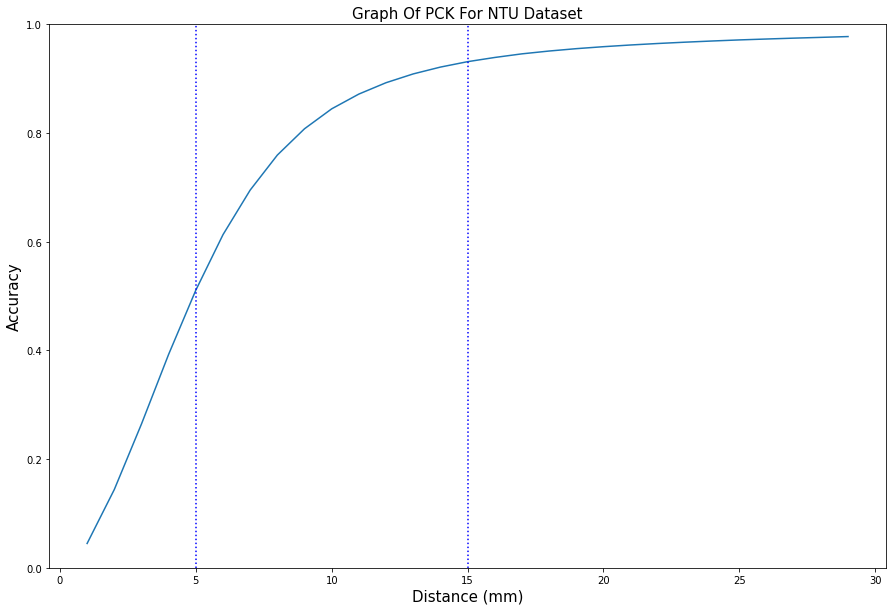
\includegraphics[width=230px]{assets/ntu_pck.png}
            \caption{NTU PCK}
            \label{fig:ntu_pck}
        \end{subfigure}
        \begin{subfigure}[b]{0.49\textwidth}
            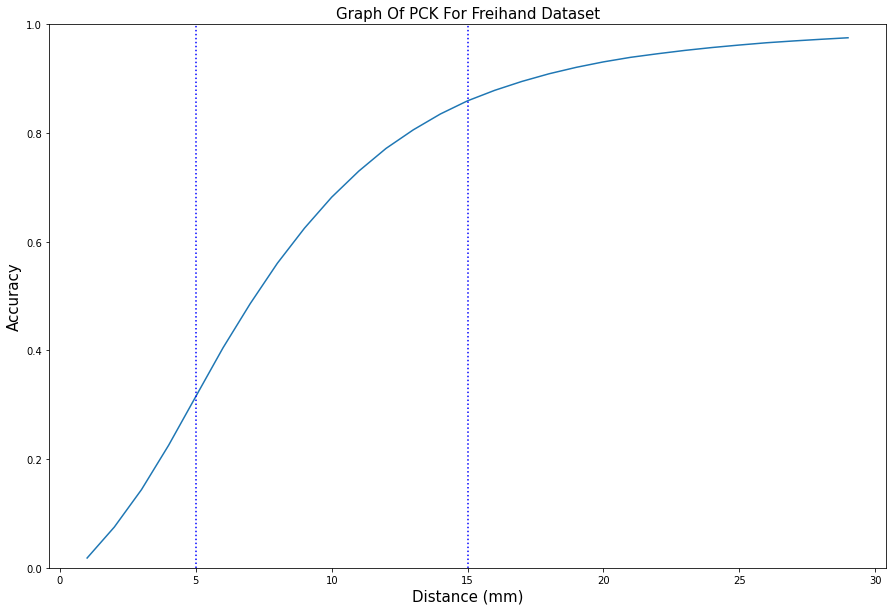
\includegraphics[width=230px]{assets/freihand_pck.png}
            \caption{Freihand PCK}
            \label{fig:freihand_pck}
        \end{subfigure}
	    \caption{Hand PCK For Different Distance Threshold}
	    \label{fig:hand_pck_for_different_thresholds}        
    \end{center}
\end{figure}


\newpage
\subsection{Body Pose Evaluation}
\noindent
Model v3.1.6 is also evaluated on the self-collected dataset for the upper body pose. Table \ref{table:model_evaluation_body_pose} shows the MPJPE, PCK@15mm, and PCK@30mm for each joint and the overall average. This table also compares to performance of v3.1.6 to that of SemGCN where the two 2D poses instead of the image encoded features were used to lift up the 2D poses to 3D.
\begin{table}[ht]
\centering
\begin{tabular*}{\textwidth}{c @{\extracolsep{\fill}} cccccc}
\toprule
Model &  \multicolumn{3}{c}{v3.1.6} & \multicolumn{3}{c}{SemGCN} \\[0.5ex] 
\midrule
{} & MPJPE & PCK@15mm & PCK@30mm & MPJPE & PCK@15mm & PCK@30mm \\ 
\hline
Neck & 8.16 & 94.20 & 100.0 & 24.59 & 42.22 & 77.84 \\ 
Spine & 13.07 & 67.02 & 99.40 & 21.43 & 47.56 & 81.13 \\
LShoulder & 14.13 & 58.02 & 98.56 & 27.72 & 25.58 & 71.29 \\
LElbow & 28.99 & 13.40 & 58.82 & 76.81 & 4.22 & 18.20 \\
LWrist & 37.28 & 9.24 & 40.22 & 93.08 & 3.36 & 16.89 \\ 
RShoulder & 15.16 & 55.73 & 96.38 & 23.49 & 39.00 & 71.13 \\
RElbow & 39.93 & 7.33 & 71.38 & 60.65 & 10.53 & 34.91 \\
RWrist & 50.72 & 7.47 & 29.87 & 80.72 & 1.13 & 9.98 \\
Average & 25.93 & 39.05 & 70.58 & 51.06 & 21.70 & 47.67 \\
[1ex] 
\hline
\end{tabular*}
\caption{Model Evaluation For Body Pose}
\label{table:model_evaluation_body_pose}
\end{table}

\begin{figure}[ht]
    \begin{center}
        \begin{subfigure}[b]{0.49\textwidth}
            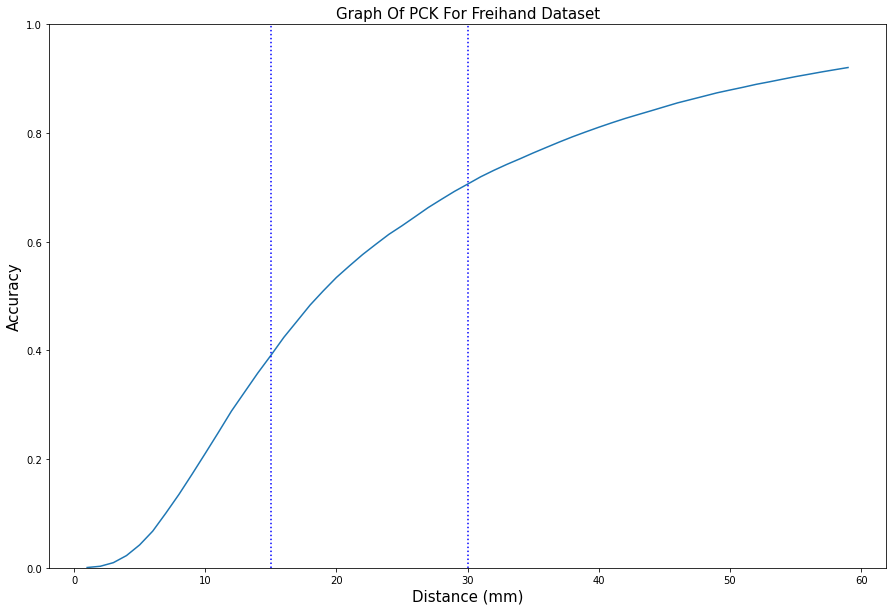
\includegraphics[width=230px]{assets/custom_pck.png}
            \caption{Model v3.1.6 PCK}
            \label{fig:custom_pck}
        \end{subfigure}
        \begin{subfigure}[b]{0.49\textwidth}
            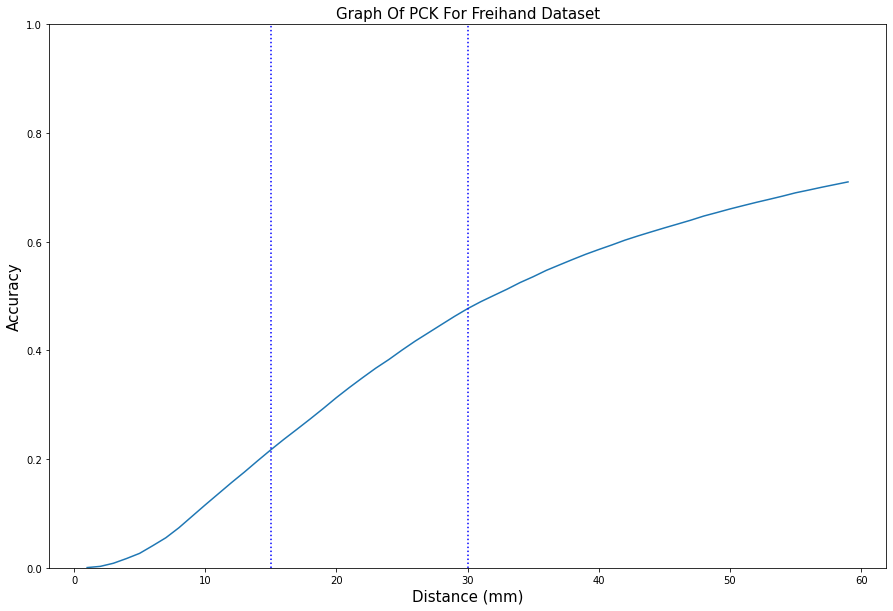
\includegraphics[width=230px]{assets/semgcn_pck.png}
            \caption{SemGCN PCK}
            \label{fig:semgcn_pck}
        \end{subfigure}
	    \caption{Body PCK For Different Distance Threshold}
	    \label{fig:body_pck_for_different_thresholds}        
    \end{center}
\end{figure}

\noindent
The metrics PCK15mm and PCK30mm is used instead of PCK5mm and PCK15mm because the 3D upper body pose covers more distance. Model v3.1.6 performs better than SemGCN because it used the image embeddings to encodes useful features that can help to resolve the ambiguity in the 2D to 3D mapping. However, the performance of v3.1.6 is worst on this upper body pose dataset than the hand pose dataset. This is mainly because the data is collected from the depth camera and cannot precisely measured the joint distance from the camera when it detects the surface of the body. This results in different bone vectors of different magnitude and direction. Figure \ref{fig:body_pck_for_different_thresholds} shows the PCK for different threshold to visualise the precision of the model in estimating the 3D pose.

\newpage
\subsection{Qualitative Results}
\noindent
This section shows Model v3.1.6 inference on the NTU and Freihand testing dataset. Figure \ref{fig:pose_2d_and_3d_on_ntu_hand} shows a sample inference on the NTU dataset that is successful. Figure \ref{fig:pose_2d_and_3d_on_freihand_hand} shows a sample inference on the Freihand dataset that is successful. The inferences shows that the model is able to predict the poses on the testing data relatively well.

\begin{figure}[ht]
    \begin{center}
        \begin{subfigure}[b]{0.32\textwidth}
            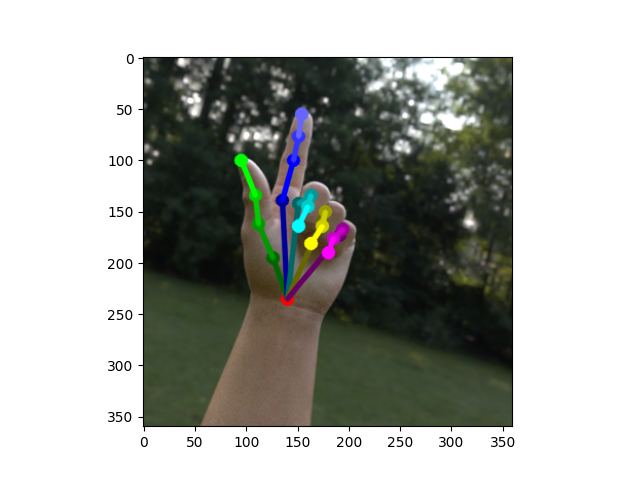
\includegraphics[width=150px]{assets/ntu_2d.png}
            \caption{2D pose}
            \label{fig:ntu_hand_2d}
        \end{subfigure}
        \begin{subfigure}[b]{0.32\textwidth}
            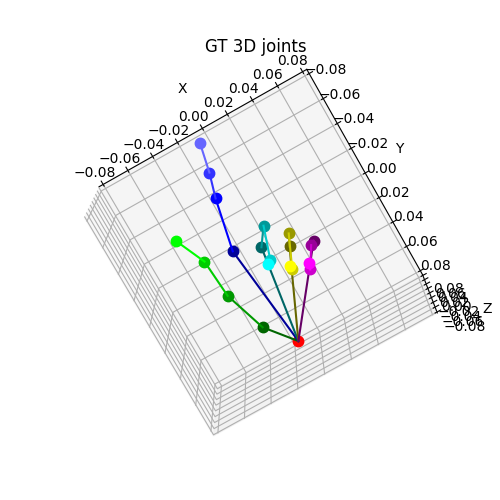
\includegraphics[width=150px]{assets/ntu_3d_gt.png}
            \caption{3D pose}
            \label{fig:ntu_hand_3d_gt}
        \end{subfigure}
        \begin{subfigure}[b]{0.32\textwidth}
            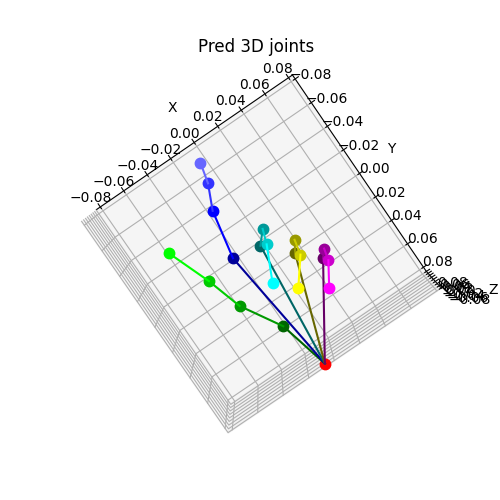
\includegraphics[width=150px]{assets/ntu_3d_pred.png}
            \caption{3D pose}
            \label{fig:ntu_hand_3d_pred}
        \end{subfigure}
	    \caption{Pose 2D and 3D estimation on NTU hand}
	    \label{fig:pose_2d_and_3d_on_ntu_hand}        
    \end{center}
\end{figure}

\begin{figure}[ht]
    \begin{center}
        \begin{subfigure}[b]{0.32\textwidth}
            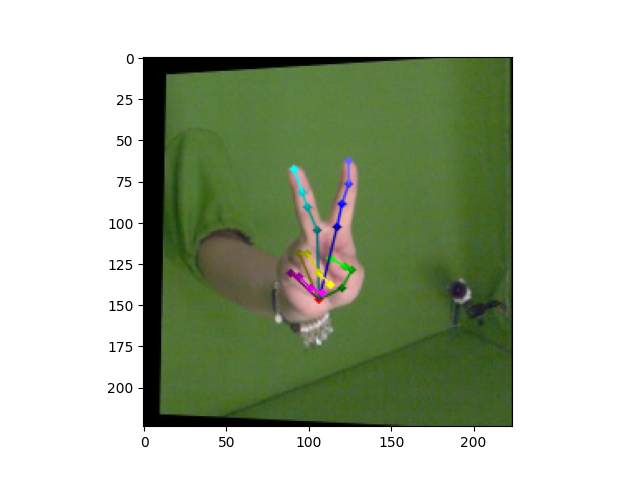
\includegraphics[width=150px]{assets/freihand_2d.png}
            \caption{2D pose}
            \label{fig:freihand_hand_2d}
        \end{subfigure}
        \begin{subfigure}[b]{0.32\textwidth}
            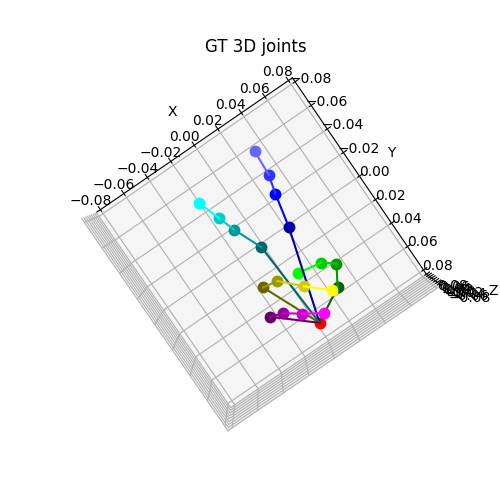
\includegraphics[width=150px]{assets/freihand_3d_gt.png}
            \caption{3D pose}
            \label{fig:freihand_hand_3d_gt}
        \end{subfigure}
        \begin{subfigure}[b]{0.32\textwidth}
            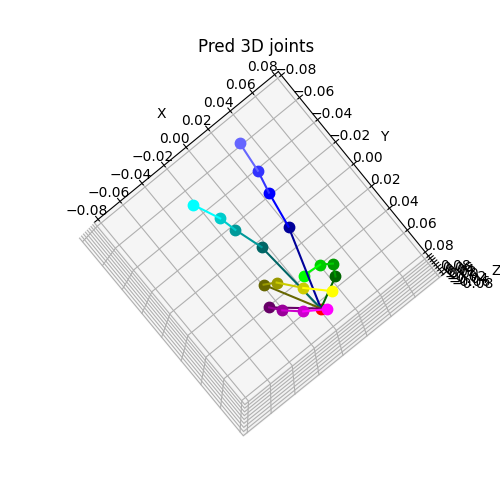
\includegraphics[width=150px]{assets/freihand_3d_pred.png}
            \caption{3D pose}
            \label{fig:freihand_hand_3d_pred}
        \end{subfigure}
	    \caption{Pose 2D and 3D estimation on Freihand hand}
	    \label{fig:pose_2d_and_3d_on_freihand_hand}        
    \end{center}
\end{figure}

\noindent
Figure \ref{fig:pose_2d_and_3d_on_real_hand} shows the pose estimation on a real hand to demonstrate that the model does not perform well on the dataset but can also generalise to other hand as well. The model can also estimate the hand pose when the hand is holding an object. The finger keypoints are important the anchor points to estimate the pose even though the palm keypoints may be occluded.

\begin{figure}[ht]
    \begin{center}
        \begin{subfigure}[b]{0.19\textwidth}
            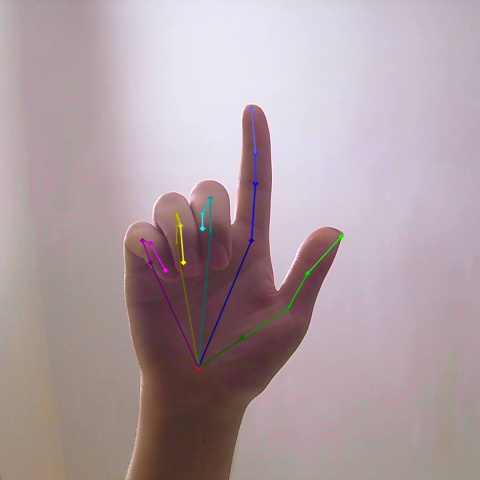
\includegraphics[width=80px]{assets/real_2d.jpg}
            \caption{2D pose}
            \label{fig:real_hand_2d}
        \end{subfigure}
        \begin{subfigure}[b]{0.21\textwidth}
            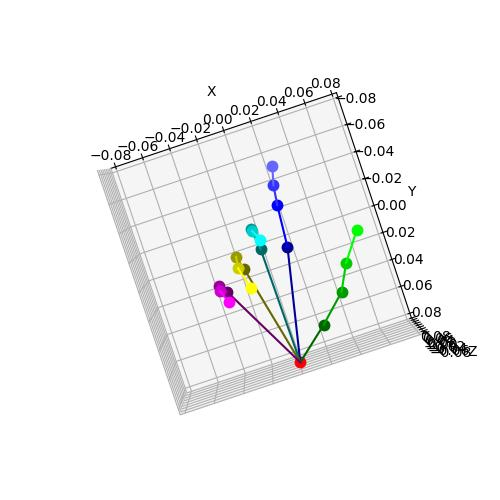
\includegraphics[width=100px]{assets/real_3d.jpg}
            \caption{3D pose}
            \label{fig:real_hand_3d}
        \end{subfigure}
        \begin{subfigure}[b]{0.19\textwidth}
            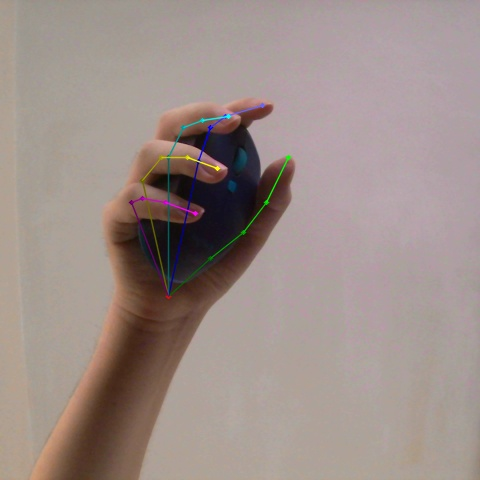
\includegraphics[width=80px]{assets/occluded_2d.jpg}
            \caption{2D Occluded}
            \label{fig:occluded_real_hand_2d}
        \end{subfigure}
        \begin{subfigure}[b]{0.21\textwidth}
            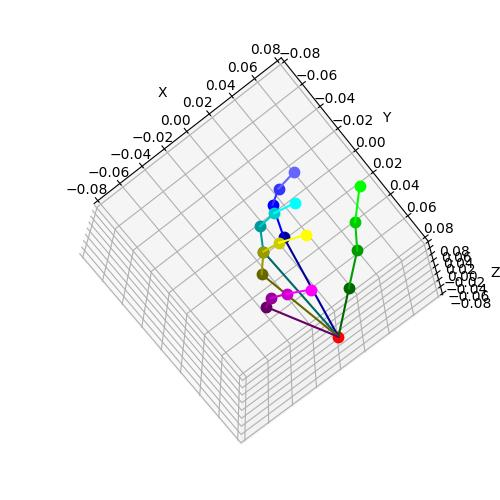
\includegraphics[width=100px]{assets/occluded_3d.jpg}
            \caption{3D Occluded}
            \label{fig:occuluded_real_hand_3d}
        \end{subfigure}
	    \caption{Pose 2D and 3D estimation on real hand}
	    \label{fig:pose_2d_and_3d_on_real_hand}        
    \end{center}
\end{figure}

\noindent
Figure \ref{fig:pose_2d_and_3d_on_failed_hand} shows a failed cased in estimating the 2d pose. However, the estimated 3d pose still has the shape of a hand. The model can give a reasonable estimation of the 3d pose from the encode features of the image. However, SemGCN that lifts the 2d pose to 3d pose cannot give reasonable estimation since the model relies solely on 2d poses.

\begin{figure}[ht]
    \begin{center}
        \begin{subfigure}[b]{0.32\textwidth}
            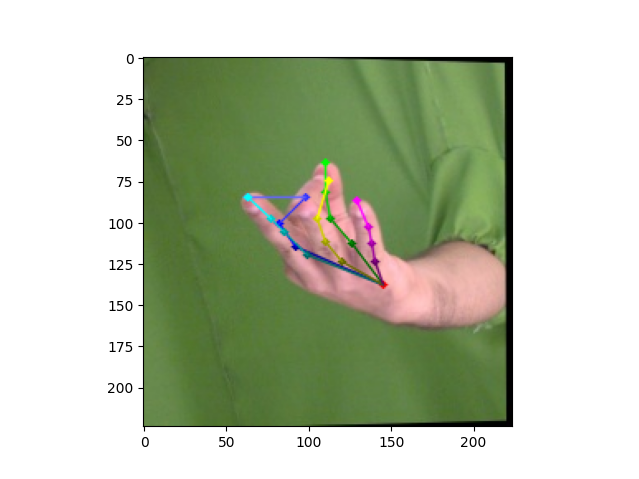
\includegraphics[width=150px]{assets/failed_2d.png}
            \caption{2D pose}
            \label{fig:failed_hand_2d}
        \end{subfigure}
        \begin{subfigure}[b]{0.32\textwidth}
            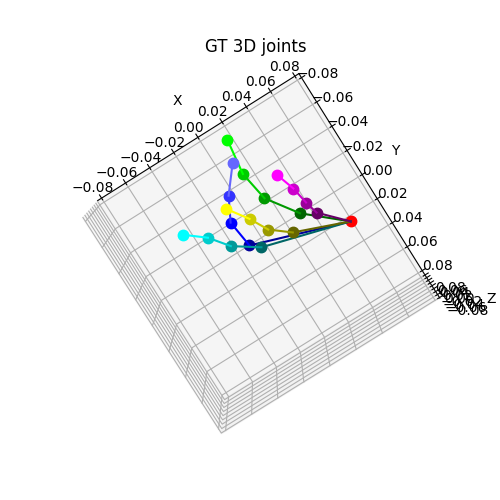
\includegraphics[width=150px]{assets/failed_3d_gt.png}
            \caption{3D pose}
            \label{fig:failed_hand_3d_gt}
        \end{subfigure}
        \begin{subfigure}[b]{0.32\textwidth}
            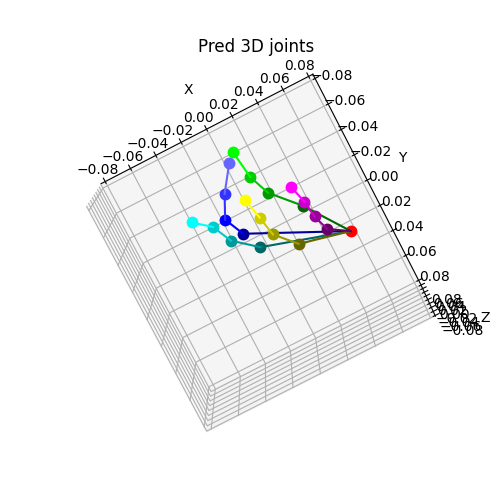
\includegraphics[width=150px]{assets/failed_3d_pred.png}
            \caption{3D pose}
            \label{fig:failed_hand_3d_pred}
        \end{subfigure}
	    \caption{Failed Pose 2D and 3D estimation on Freihand hand}
	    \label{fig:pose_2d_and_3d_on_failed_hand}        
    \end{center}
\end{figure}


\newpage
\subsection{Robotic Arm Teleoperation}
\noindent
After training the pose estimation models, the models were integrated with the robotic arm setup to demonstrate a pick-and-place action. The orientation of the hand is computed from three joints on the palm (Index 1, Pinky 1, and Wrist) to control the orientation of the end effector. The gripper state is computed from the distance between the index tip and the thumb tip (Index 4 and Thumb 4) to open and close the gripper. The position of the end effector is computed from the relative displacement from the initial position of the wrist joint. However, in simulation, it was observed that the position end effector was difficult to control because the upper body pose estimation model was not very precise. Object detection was used instead to track the center of the hand in the image. The displacement of the center of the hand from the center of the image was mapped to the position of the end effector.

\noindent
Figure \ref{fig:pick_and_place_demo} shows the pick and place demonstration in the physical environment. The image on the left is a screen recording that shows the objection detection and pose estimations. It also shows the simulation for testing. The image on the right shows the video recording on the physical robot where the goal is to pick the orange cube and place on the white plate. The cube was picked with the end effector orientated inwards because the robotic arm extends beyond the cube location. The hand shows that the finger and thumb is closed together, corresponding to the closed gripper state. The end effector hovered over the white plate before the cube was released by spreading the thumb and index finger.
\begin{figure}[ht]
	\begin{center}
		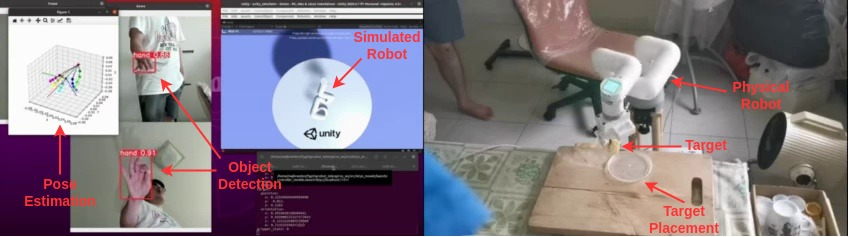
\includegraphics[width=450px]{assets/pick_and_place.jpg}
		\caption{Pick And Place Demonstration}
		\label{fig:pick_and_place_demo}
	\end{center}
\end{figure}

\newpage
\section{Conclusion}
\noindent
This project successfully designed and trained 3D pose estimation from scratch for the upper body pose and hand pose. This project also demonstrated the use of hand pose estimation model to control the orientation of the end effector. However, the body pose estimation model was still not robust enough to control the position of the end effector. Instead of the body pose estimation model, hand object detection model was used as an alternative.

\noindent
One limitation of the pose estimation models in this project is that it works on 1 hand or 1 upper body in the image. This allows the model to be lightweights and is sufficient for the scope of this project. Another limitation of the models is that the model cannot perform well under high occlusion, such as the hand is perpendicular to the image plane. The 3d hand pose will appear compact and squashed.

\noindent
There are room for improvements for this lightweight models. One improvements is to perform model distillation where a large image encoder such as ResNet50 is used to extract image features and a small image encoder such as ResNet18 learns the encoded embeddings. The number of channels in the ResNet architecture can also be reduced. Since the model trained on synthetic hand dataset can generalize to the real data, the same method can be used for the body pose estimation to reduce the need for manual annotation.

\noindent
This project shows that 3D pose estimation to teleoperate the robotic arm is feasible to some extent. However, there might be easier ways to control the robotic arm, such as using object detection instead of body pose estimation. As a note for future developments, a mobile phone can be used instead. Most mobile phone has IMU sensors that can give accurate position and orientation. However, the camera can be used to determine the finger pose instead to grasp the object to reduce the need for complicated hardware. The phone can vibrate to provide some form of tactile feedback. This reduce the device needed to only the mobile phone for the setup.


\newpage
\section{References}
\printbibliography[heading=none]

\newpage
\section{Appendix}
\subsection{Upper Body Skeleton}
\noindent
The skeleton and the corresponding names for each joint for the upper body are illustrated in Figure \ref{fig:upper_body_skeleton} and Table \ref{table:upper_body_joint_names} respectively. There are 8 keypoints.
\begin{table}[ht]
\begin{minipage}[b]{0.60\linewidth}
\centering
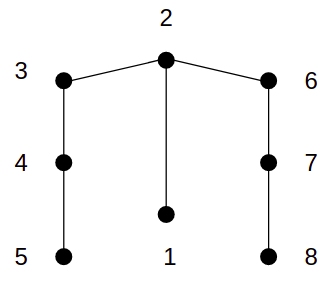
\includegraphics[width=250px]{assets/upper_body_skeleton.png}
\captionof{figure}{Upper Body Skeleton}
\label{fig:upper_body_skeleton}
\end{minipage}
\begin{minipage}[b]{0.35\linewidth}
\centering
\begin{tabular*}{\textwidth}{ c @{\extracolsep{\fill}} p{1.5in}}
Index & Joint Name \\ \hline
1 & Spine  \\ 
2 & Neck  \\ 
3 & Right Shoulder  \\ 
4 & Right Elbow  \\ 
5 & Right Wrist  \\ 
6 & Left Shoulder  \\
7 & Left Elbow  \\ 
8 & Left Wrist  \\ 
\end{tabular*}
\caption{Upper Body Joint Names}
\label{table:upper_body_joint_names}
\end{minipage}\hfill
\end{table}
\newpage

\subsection{Hand Skeleton}
\noindent
The skeleton and the corresponding names for each joint for the hand are illustrated in Figure \ref{fig:hand_skeleton} and Table \ref{table:hand_joint_names} respectively. There are 21 keypoints.
\begin{table}[ht]
\begin{minipage}[b]{0.60\linewidth}
\centering
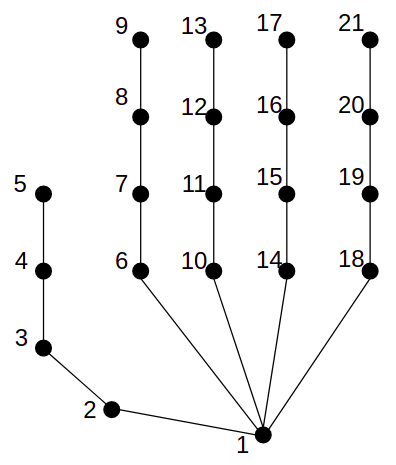
\includegraphics[width=250px]{assets/hand_skeleton.png}
\captionof{figure}{Hand Skeleton}
\label{fig:hand_skeleton}
\end{minipage}
\begin{minipage}[b]{0.35\linewidth}
\centering
\begin{tabular*}{\textwidth}{ c @{\extracolsep{\fill}} p{1.5in}}
Index & Joint Name \\ \hline
1 & Wrist  \\ 
2 & Thumb 1  \\ 
3 & Thumb 2  \\ 
4 & Thumb 3  \\ 
5 & Thumb 4  \\ 
6 & Index 1  \\
7 & Index 2  \\ 
8 & Index 3  \\ 
9 & Index 4  \\ 
10 & Middle 1   \\ 
11 & Middle 2  \\ 
12 & Middle 3  \\ 
13 & Middle 4  \\ 
14 & Ring 1  \\
15 & Ring 2  \\ 
16 & Ring 3  \\ 
17 & Ring 4  \\ 
18 & Pinky 1  \\ 
19 & Pinky 2  \\ 
20 & Pinky 3  \\ 
21 & Pinky 4  \\ 
\end{tabular*}
\caption{Hand Joint Names}
\label{table:hand_joint_names}
\end{minipage}\hfill
\end{table}

\end{document}
